%----------------------------------------------------------------------------------------
%	PACKAGES AND OTHER DOCUMENT CONFIGURATIONS
%----------------------------------------------------------------------------------------

\documentclass[11pt,a4paper]{article}

%\usepackage{blindtext} % Package to generate dummy text throughout this template 

% \usepackage[sc]{mathpazo} % Use the Palatino font
\usepackage[T1]{fontenc} % Use 8-bit encoding that has 256 glyphs
\linespread{1.05} % Line spacing - Palatino needs more space between lines
\usepackage{microtype} % Slightly tweak font spacing for aesthetics

\usepackage[english]{babel} % Language hyphenation and typographical rules

\usepackage[hmarginratio=1:1,top=32mm,columnsep=20pt]{geometry} % Document margins
\usepackage[hang, small,labelfont=bf,up,textfont=it,up]{caption} % Custom captions under/above floats in tables or figures
\usepackage[usenames,dvipsnames,svgnames,table]{xcolor}

\usepackage{booktabs} % Horizontal rules in tables

\usepackage{lettrine} % The lettrine is the first enlarged letter at the beginning of the text

\usepackage{enumitem} % Customized lists
\setlist[itemize]{noitemsep} % Make itemize lists more compact

\usepackage{abstract} % Allows abstract customization
\renewcommand{\abstractnamefont}{\normalfont\bfseries} % Set the "Abstract" text to bold
\renewcommand{\abstracttextfont}{\normalfont\small\itshape} % Set the abstract itself to small italic text

\usepackage{titlesec} % Allows customization of titles
% \renewcommand\thesection{\Roman{section}} % Roman numerals for the sections
% \renewcommand\thesubsection{\roman{subsection}} % roman numerals for subsections
% \titleformat{\section}[block]{\large\scshape\centering}{\thesection.}{1em}{} % Change the look of the section titles
% \titleformat{\subsection}[block]{\large}{\thesubsection.}{1em}{} % Change the look of the section titles

\usepackage{fancyhdr} % Headers and footers

\usepackage{titling} % Customizing the title section

\usepackage{hyperref} % Hyperlinks in the PDF

\usepackage{graphicx}
\usepackage{tocloft}
\usepackage{dsfont}

\usepackage{amsthm}

\usepackage{tikz} % Graphics package
\usetikzlibrary{positioning, fit}
\usetikzlibrary{arrows.meta, shapes.geometric}

\usepackage{graphviz}

\usepackage{preview}

\usepackage{multirow} % Multirow tables support
\usepackage{longtable} % Long tables support

\usepackage{todonotes}

\usepackage{xspace} % for spaces after user-defined commands

\usepackage{mathtools} % for math notation
\usepackage{amsfonts} % for math notation
\usepackage{amssymb} % for math notation

\usepackage[linesnumbered,ruled,vlined,noend]{algorithm2e}

\usepackage{enumitem} % fix breaking lines in enums

\usepackage{alltt}
\usepackage{float}

%%% Page align %%%
\geometry{a4paper,top=2cm,bottom=2cm,left=3cm,right=2cm}

%%%Encoding and fonts%%%


%%% Paragraphs align %%%
\sloppy
\clubpenalty=10000
\widowpenalty=10000	

%%%Bibliography%%%
\makeatletter
\bibliographystyle{ieeetr}
\makeatother

%%%Images%%%
\graphicspath{{images/}}

%%% Hyperlinks colors %%%
\definecolor{linkcolor}{rgb}{0.9,0,0}
\definecolor{citecolor}{rgb}{0,0.6,0}
\definecolor{urlcolor}{rgb}{0,0,1}
\hypersetup{
    colorlinks, linkcolor={linkcolor},
    citecolor={citecolor}, urlcolor={urlcolor}
}

%%% Theorem styles definitions %%%

\theoremstyle{definition}
\newtheorem{definition}{Definition}

\theoremstyle{remark}
\newtheorem*{remark}{Remark}

%%% FancyHDR styles definitions %%%
\pagestyle{fancy} % All pages have headers and footers
\fancyhead{} % Blank out the default header
\fancyfoot{} % Blank out the default footer
\fancyhead[C]{=nil;'s zkSharding for Ethereum} % Custom header text
\fancyfoot[RO,LE]{\thepage} % Custom footer text

\reversemarginpar % for correct TODO work

%\renewcommand{\todo}[5][4]{\ignorespaces}  %% uncomment this to hide all TODOs

\newcommand{\nil}{\texttt{=nil;}\xspace}
\newcommand{\protocol}{\texttt{=nil;} zkSharding\xspace}
\newcommand{\evm}{\texttt{=EVM++;}\xspace}
\newcommand{\stakemarket}{Stake Market\xspace}

\newcommand{\set}[1]{{\ensuremath{\mathcal{#1}}}}
\newcommand{\algo}[1]{\ensuremath{\textsc{#1}}}
\newcommand{\bhead}{\mathsf{bh}}
\newcommand{\block}{\mathsf{B}}
\newcommand{\chain}{\mathfrak{C}}
\newcommand{\tx}{\mathsf{tx}}
\newcommand{\ctx}{\mathsf{c}\tx}

\newcommand{\st}{\mathsf{st}}
\newcommand{\stroot}{\mathsf{s}}
\newcommand{\hash}{\mathsf{hash}}

\newcommand{\val}{\mathsf{V}}
\newcommand{\user}{\mathsf{U}}
\newcommand{\valset}{\set{V}}
\newcommand{\stake}{\mathsf{st}}
\newcommand{\ratiolarge}{\eta}
\newcommand{\ratioLexe}{\theta}
\newcommand{\largeval}{\valset^{>}}
\newcommand{\smallval}{\valset^{<}}
\newcommand{\lmin}{\ensuremath{\ell_{min}}}
\newcommand{\distance}{\Delta}

\newcommand{\kzg}{\mathsf{Com}_{da}}
\newcommand{\fri}{\mathsf{Com}_{tx}}
\newcommand{\stateproof}{\mathsf{\pi_{st}}}
\newcommand{\polykzg}{\mathsf{P}_{kzg}}
\newcommand{\polyfri}{\mathsf{P}_{fri}}

\newcommand{\txlist}{\set{T}}

\newcommand{\shard}{\mathbb{S}}

%ALGOS

\newcommand{\commitpoly}{\algo{CommitPoly}}
\newcommand{\updatestate}{\algo{UpdateState}}

\newcommand{\outbox}{\mathcal{O}}

\newcommand{\sender}{S}
\renewcommand{\to}{\mathsf{to}}
\newcommand{\data}{\mathsf{data}}
\newcommand{\sid}{\mathsf{sid}}

\newcommand{\syncSet}{\set{SC}}
\newcommand{\fzkvm}{\mathsf{F_{zkvm}}}
\newcommand{\batch}{\mathcal{B}}
\newcommand{\fstf}{\mathsf{F}}
\newcommand{\combatch}{\mathsf{Com}_\batch}
\newcommand{\commit}{\algo{Commit}}
\newcommand{\mtroot}{\algo{Root}}
\newcommand{\compress}{\algo{Compress}}
\newcommand{\prover}{\mathsf{P}}
\newcommand{\circuit}{\mathcal{C}}
\setlength{\droptitle}{-4\baselineskip} % Move the title up

\pretitle{
    \begin{center}
    \end{center}
} % Article title formatting
\title{
    \begin{center}
        \Huge\bfseries {zkSharding Solution Brief}
    \end{center}
} % Article title
\posttitle{
    \begin{center}
        %        \Large\bfseries What is next? \\
    \end{center}
} % Article title closing formatting
%\author{%
%    \textsc{Author Name} \\[1ex] % Your name
%    \normalsize \texttt{=nil;} Foundation \\ % Your institution
%    \normalsize \href{mail}{mail} % Your email address
%    \and 
%}
\date{\today} % Leave empty to omit a date
% \renewcommand{\maketitlehookd}{%
%     \begin{abstract}
%         \noindent 
%     \end{abstract}
% }

\def\short#1#2{#1} %to make shorter version of the document, use #1, otherwise #2
\newcommand{\handan}[1]{{\color{red}\textsc{Handan:} #1}}
\newcommand{\alex}[1]{{\color{blue}\textsc{Aleksandar:} #1}}
\begin{document}

% Print the title
\maketitle

%\tableofcontents
\clearpage


\section{Introduction}
\label{section:introduction}

The imperative to scale Ethereum is driven by its growing user base and the 
increasing complexity of applications built on its platform. The current 
strategy to address the scaling issues leans heavily on the concept of modularity 
through rollups and data availability and consensus layers.

While this approach has shown promise, existing solutions introduce several drawbacks:
\begin{itemize}
    \item \textbf{Fragmentation}:
      Rollups are separated from each other by design. 
      This leads to fragmentation in terms of security, liquidity, and data consistency.
    \item \textbf{Updates in zkEVMs}:
        The dynamic nature of zkEVMs brings regular updates that may lead 
        to potential security vulnerabilities.
    \item \textbf{Applications Redeployments}:
        Users have to redeploy their applications from Ethereum to L2, which in
        the same time causes liquidity fragmentation which leads us to the first
        point. 
\end{itemize}

In addressing Ethereum's scalability and fragmentation challenges, 
we propose a new layer-2 (L2) concept, \textit{zkSharding}.
This solution merges Zero-Knowledge proofs with a sharding mechanism and blends 
a bunch of other \nil technologies into it. 

Key aspects include:
\begin{itemize}
    \item \textbf{"zkRollup with Sharding" for Horizontal Scalability}:
    The core of zkSharding is a blend of zkRollups and sharding, enabling extensive 
    horizontal scalability without compromising security or reducing efficiency. 
    This approach counters the limitations of vertical scaling (L3, L4, etc.),
    significantly reducing data and liquidity fragmentation.
    \item \textbf{Direct Ethereum data access}:
    The ability to call Ethereum's original data from L2 applications allows us 
    to reuse already deployed applications. Direct access to L1 data from L2 
    ensures a more unified and seamless environment.
    \item \textbf{Type-1 zkEVM Compiled via zkLLVM from in-Production EVM}:
        zkEVM's, being often implemented from scratch to replicate the actual
        state transition executor logic (EVM) pose security risks as the circuit
        is very large, very complicated and hardly auditable. zkSharding relies
        on a zkEVM circuit compiled by zkLLVM circuit compiler from a 
        production-grade EVM without manual circuit reimplementation which
        reduces security risks.
\end{itemize}

We envision zkSharding as a step forward in blockchain modularity, aligning with 
Ethereum's principles and offering a scalable, integrated solution.

\nil zkSharding solution provides the follwing properties:
\begin{enumerate}
    \item \textbf{Scalability}: 
    \begin{enumerate}
        \item No scalability limitations as the execution is parallel. 
        Throughput around ~60k transfers per second with around 400
        nodes.
        \item Competitive marketplace-based proof generation guarantees
        fastest L1-finality and chepest generation costs.
    \end{enumerate}
    \item \textbf{Unified Liquidity/Security}:
    \begin{enumerate}
        \item No security/liquidity fragmentation as each shard is
         a part of the wholistic cluster. 
        \item Reduction of a need to migrate liquidity from Ethereum as
        \texttt{=nil;} provides transparent access to its' data for
        applications.
    \end{enumerate}
    \item \textbf{Security}:
    \begin{enumerate}
        \item State transitions secured by \texttt{=nil;}'s 
            zkEVM compiled via zkLLVM.
            It provides auditable security (e.g. constraints security) as the code is 
            easily inspectable since zkEVM circuits are compiled from a 
            production-used EVM implementation in high-level language
            and not written manually.
        \item Liveness security guaranteed with native staking or restaking existing staking pools (e.g. Lido) TVL.
        \item Decentralized from day one thanks to combination of Ethereum staking and Proof Market.
            See Section \ref{section:proof-market} for details.
    \end{enumerate}
    \item \textbf{Functionality}:
    \begin{enumerate}
        \item A Type-1 zkEVM\footnote{
            \url{https://vitalik.ca/general/2022/08/04/zkevm.html}
        }, fully EVM bytecode-equivelent.
        \item An environment tailored for applications 
            that have high demands related to time, memory, 
            and algorithmic complexity. 
            Examples include Decentralized Exchanges (DEXes) 
            or Proof Market\footnote{\url{proof.market}}.
    \end{enumerate}
\end{enumerate}

% \todo[inline]{May be it would be a good idea to show how it works from the client DApp point of view. 
% May be highlight some important cases, such as redeploing existing Eth contracts, for instance.
% Also, we could talk a little bit more about features, which required by DEX or any other types of clients if we understand them. S.K.}

\subsection{Overview}

As illustrated in Figure \ref{figure:overview}, 
the state of \protocol is partitioned into the main shard and several secondary 
shards. The main shard's role is to synchronize and consolidate data from the 
secondary shards. It uses Ethereum both as its Data Availability Layer and as a 
verifier for state transition proofs, similar to typical zkRollups operations. 
For a comprehensive understanding of the sharding approach, refer to Section 
\ref{section:sharding}.

Secondary shards function as "workers", executing user transactions. 
These shards maintain unified liquidity and data through a cross-shard messaging 
protocol, eliminating any fragmentation amongst them. 

Each shard is supervised by a committee of validators. There is a periodic 
rotation of these validators across shards. In addition, updates to a shard's 
state are verified to the main shard using zkEVM (see \ref{section:zkvm} for a 
detailed explanation).

Users have direct access to Ethereum data, thanks to the Ethereum Data Provider 
linked to every shard. This data is validated using zkBridge.

\begin{figure}[h]
    \centering
	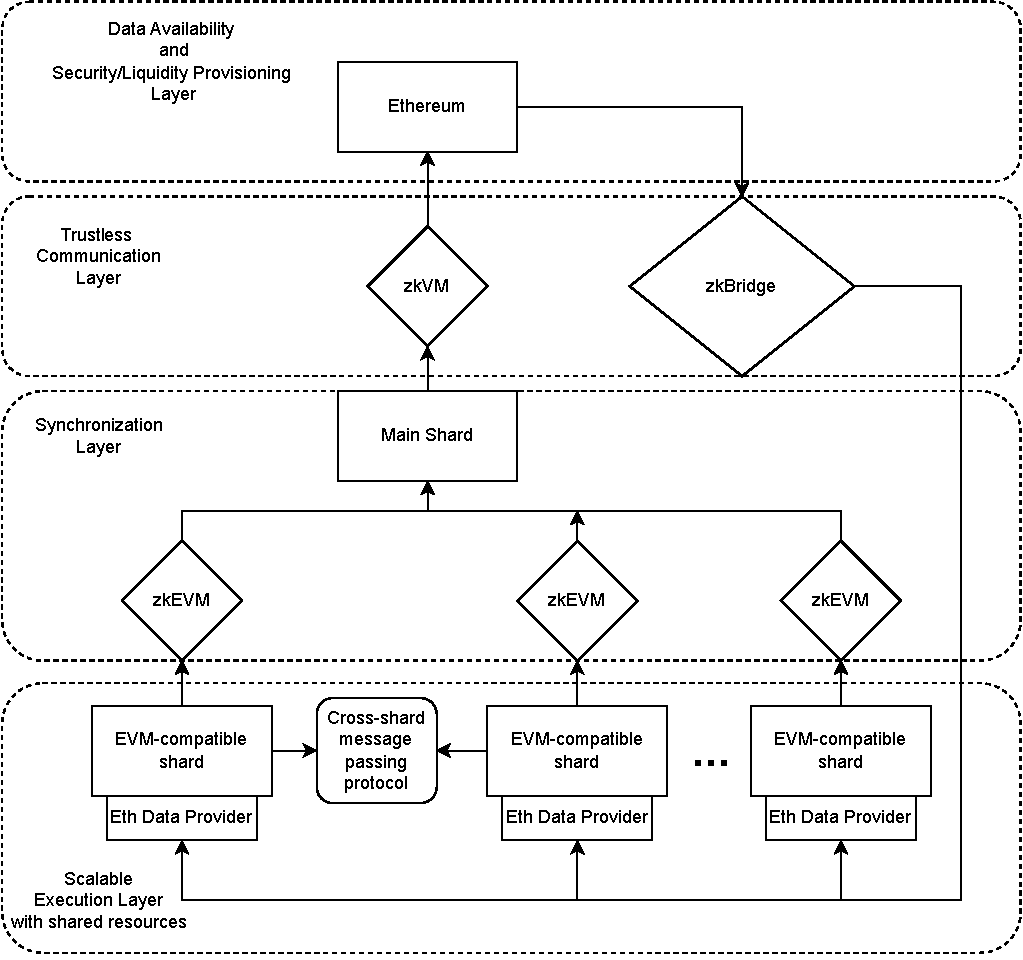
\includegraphics[scale=0.55]{figures/overview.pdf}
    \caption{\protocol overview}
     \label{figure:overview}
\end{figure}

To illustrate the transaction flow from initiation 
 by a user to confirmation on Ethereum, consider the following steps:
\begin{enumerate}
    \item The user signs a transaction $tx$ and dispatches it to the network.
    \item Validators in shard $S$, where the user's wallet is located,
        place $tx$ into the mempool.
    \item These validators then create a new block $B_{S}^{1}$.
    \item The hash of $B_{S}^{1}$ is recorded on the main shard within block $B_{M}^{1}$.
    \item A state transition proof for $B_{S}^{1}$ is 
        produced and verified by the main shard in block $B_{M}^{2}$.
    \item A state transition proof for $B_{M}^{2}$
        is sent to Ethereum for verification 
        and coupled with the necessary data for ensuring data availability.
    \item Once this process is complete, 
        $tx$ achieves confirmation by Ethereum.
\end{enumerate}

This outline assumes that the user's transaction does not
 activate the cross-shard messaging protocol.
However, in this case the transaction flow remains the same with a 
 difference that user's transaction triggers a creation of new 
 transactions on other shards. 

% \section{L1 Support in zkSharding: Contracts and Data Availability}
\subsection{L1 Support in zkSharding}
\label{sec:l1}

\todoisinline{We're going directly to typical L2-L1 communication here. I
	think, second section shoud be more related to uniqueness of our
	project

	\handan{Now, it as a subsection of the Overview section}}

\begin{figure}
	\centering
	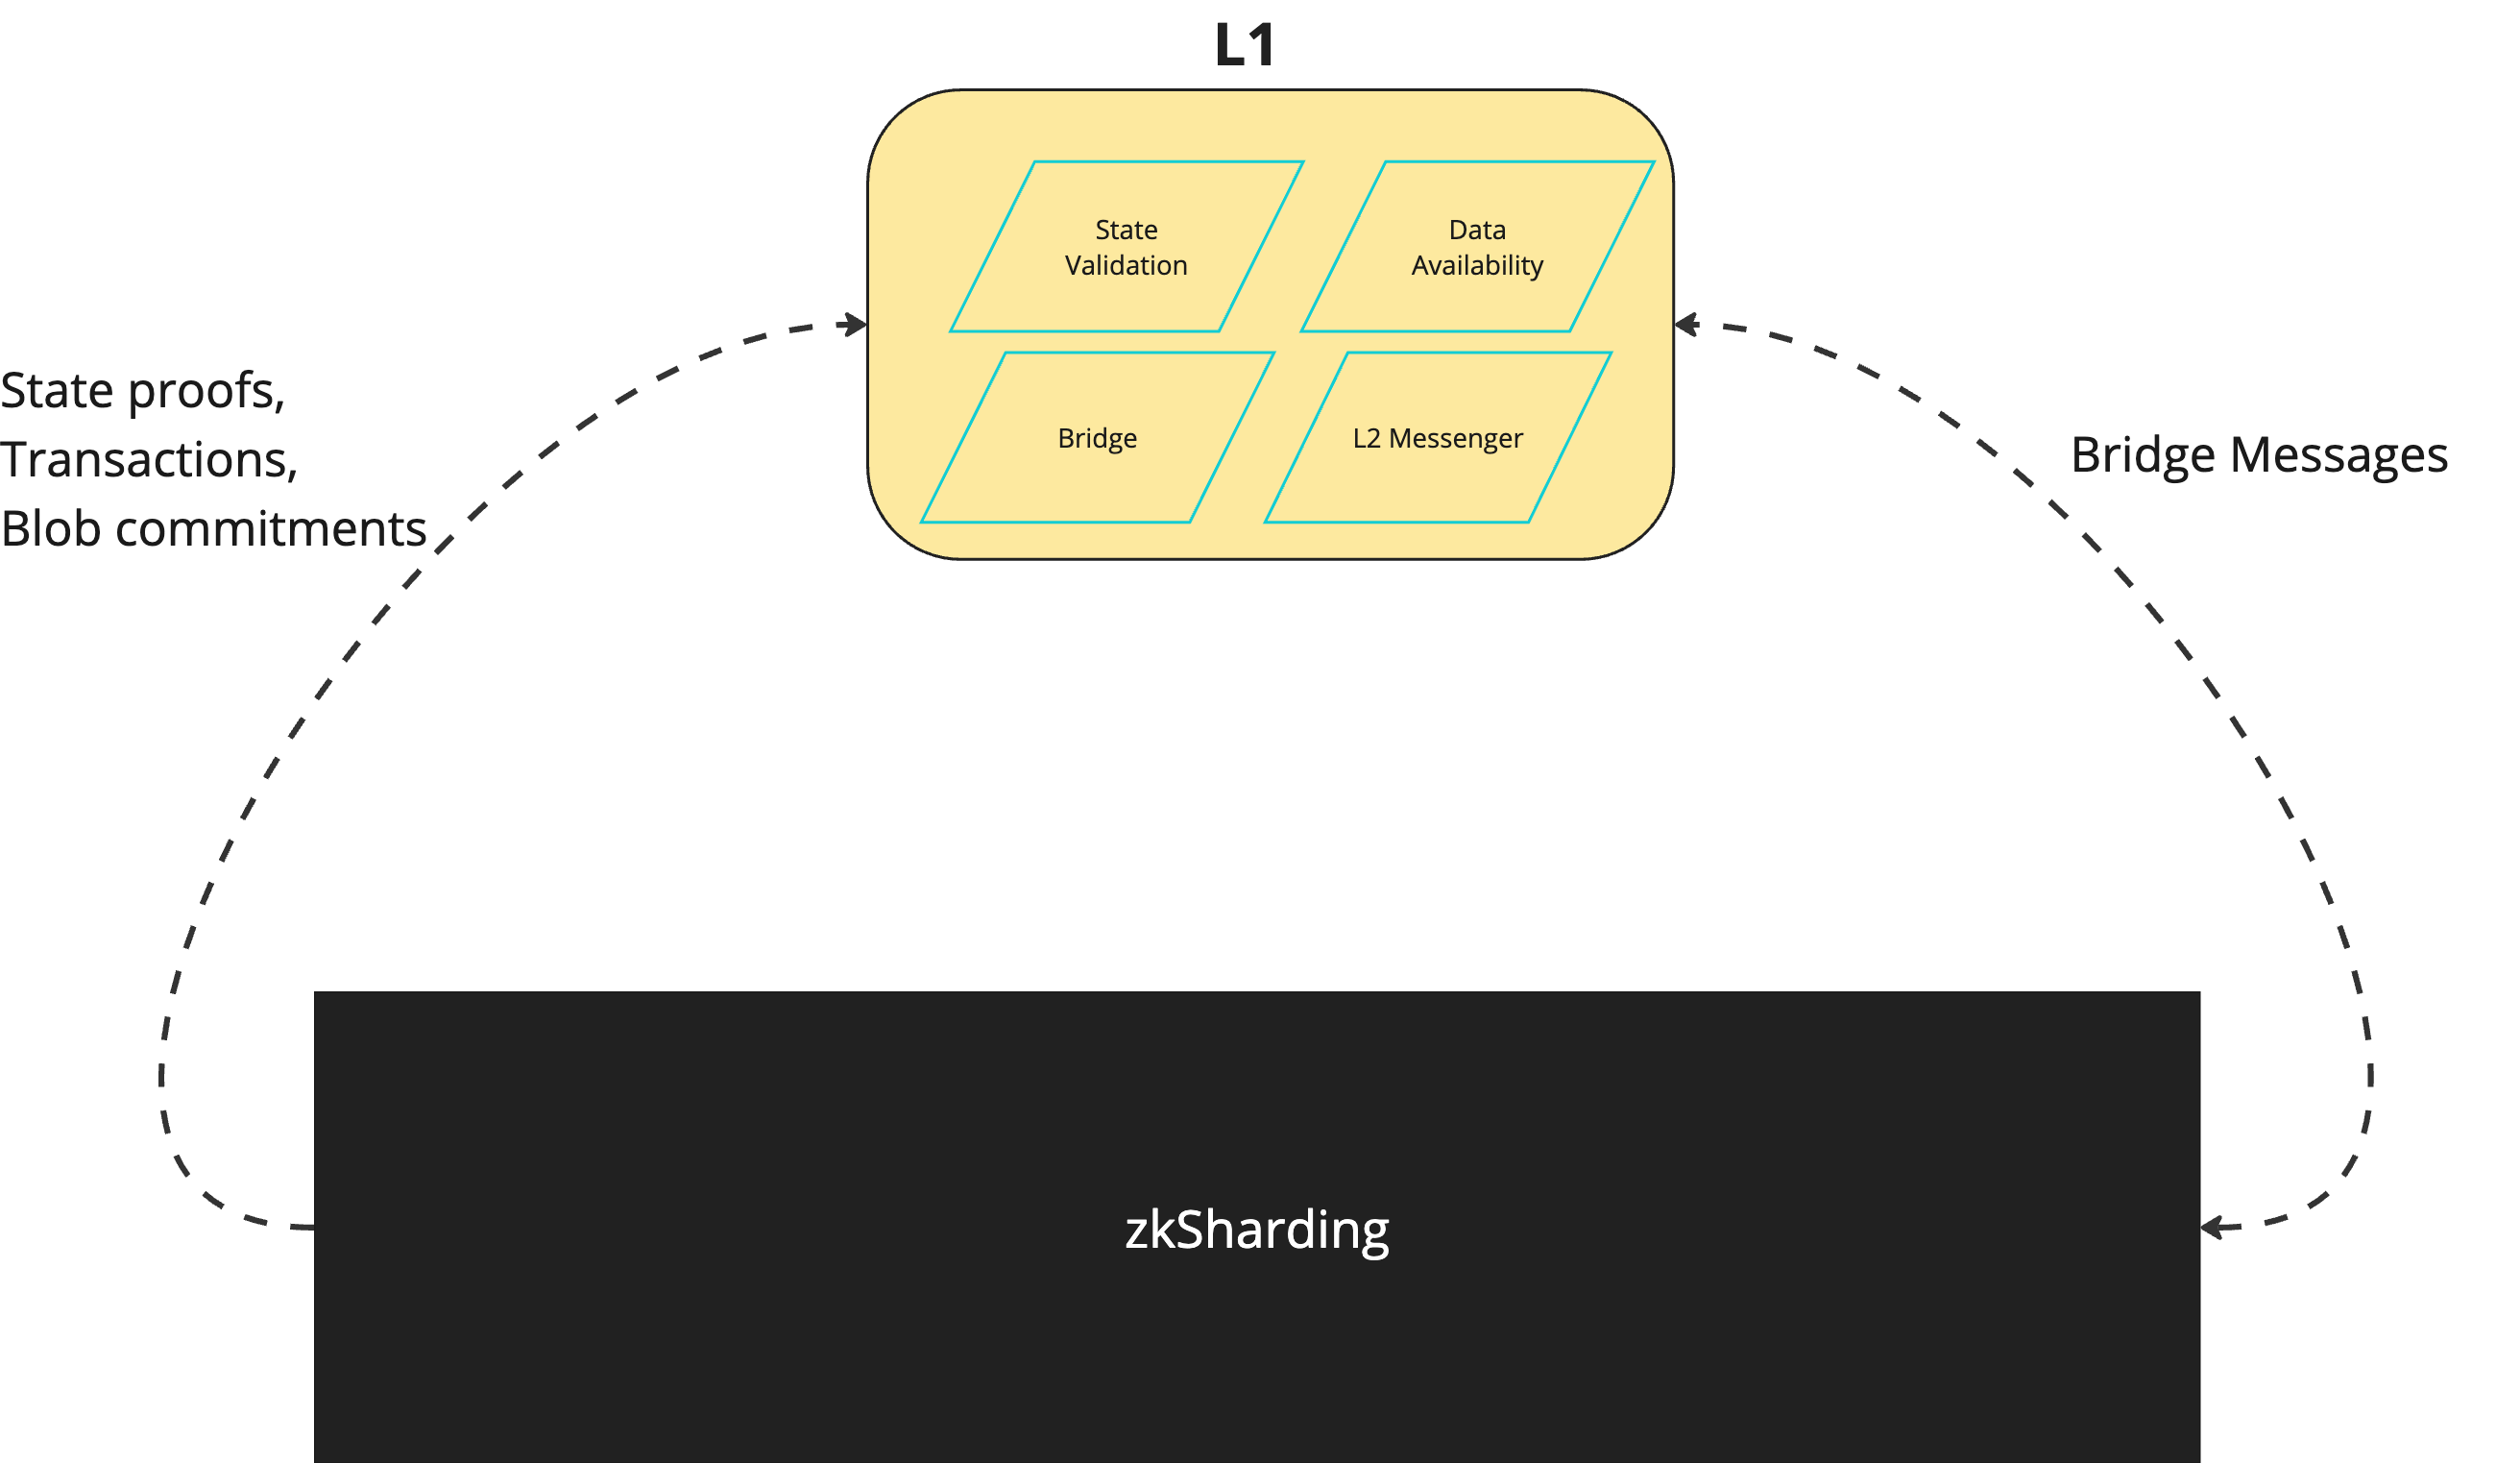
\includegraphics[width=0.5\linewidth]{figures/blackbox}
	\caption{Visualizing zkSharding as a \emph{blackbox}}
	\label{fig:blackbox}
\end{figure}

\short{
	From L1’s perspective (see
	Figure
	\ref{fig:blackbox}), zkSharding is a blackbox which periodically
	submits
	cryptographic proofs and data blobs to verify its operations
	without
	revealing internal processes. L1 provides key contracts for state
	validation, deposits, withdrawals, and data availability. While L1
	provides zkSharding with a reliable settlement layer to verify
	zkSharding's state  and a data availability layer, zkSharding
	enables L1
	to achieve higher throughput by offloading transaction processing
	to
	zkSharding. The L1 network is unaware of the detailed execution
	inside
	zkSharding, but it plays a crucial role in maintaining
	zkSharding’s
	trustworthiness and security.
}{
	Before exploring the design of zkSharding, it is crucial to
	understand
	how zkSharding functions as a rollup on Ethereum’s Layer 1 (L1).
	While
	zkSharding is internally complex, involving multiple shards
	processing
	transactions in parallel, L1 sees zkSharding much like any other
	zkRollup.
	From L1’s perspective, zkSharding periodically submits
	cryptographic
	proofs to verify the correctness of its operations and stores some
	essential data as blobs, without exposing its internal processes.
	Even though L1 is not aware of zkSharding's full internal
	operations or
	shard structure, L1 hosts key contracts that enable zkSharding’s
	integration with Ethereum, including  state validity and handling
	deposits
	and withdrawals. It also provides data availability services to
	the
	zkSharding. While L1 provides zkSharding with a reliable
	settlement layer
	to verify zkSharding's state  and act as a data availability
	layer,
	zkSharding enables L1 to achieve higher throughput by offloading
	transaction processing to zkSharding.
	In essence, one can visualize zkSharding as a \emph{blackbox} (See
	Figure
	\ref{fig:blackbox}) that processes numerous transactions and
	periodically
	submits proofs to L1 for validation. L1 verifies these proofs and
	stores
	essential data, ensuring that zkSharding remains secure and that
	users can
	transfer assets in and out of the system seamlessly. The L1
	network is
	unaware of the detailed execution inside zkSharding, but it plays
	a
	crucial role in maintaining zkSharding’s trustworthiness and
	security.
}

For more insights into zkSharding's internal mechanics and how it achieves
high throughput, refer to the next sections. Now, we introduce the key
functionalities that L1 provides to support zkSharding.

\paragraph{L1 Data Availability:}
\short{
	Proto-Danksharding (EIP-4844) \cite{eip-4844}  is a proposal aimed
	at reducing rollup costs when posting data to Ethereum’s L1.
	zkSharding
	leverages this by utilizing Ethereum's data availability layer.
	zkSharding
	submits executed transactions as a \emph{compressed} batch,
	denoted as
	$\batch^*$, in the form of a data blob. This blob is committed to
	Ethereum’s execution layer via a KZG commitment  \cite{kzg}, which
	represents the data as a polynomial for efficient storage and
	verification. Batch compression is utilized to maximize the number
	of
	transactions that can be efficiently stored within a single blob,
	ensuring
	optimal use of available space.
}{
	Proto-Danksharding (EIP-4844) \cite{eip-4844} is a proposal aimed
	at reducing rollup costs when posting data on Ethereum’s L1.
	zkSharding
	takes advantage of this by utilizing Ethereum's data availability
	layer.
	zkSharding submits the executed transactions, referred to as the
	compressed batch $\batch^*$, in the form of a data blob, which is
	then
	committed to L1’s execution layer using a KZG commitment. A KZG
	commitment
	\cite{kzg} is a cryptographic method that allows Ethereum to
	efficiently
	verify large amounts of data (such as zkSharding’s transaction
	history) by
	representing the blob data as a polynomial. This ensures efficient
	data
	storage while maintaining the ability to verify that zkSharding’s
	transactions are available and valid. zkSharding uses batch
	compression to
	maximize the number of transactions that can be efficiently stored
	within
	a single blob, ensuring optimal use of available space
	\cite{compression}.
}

\paragraph{State Validity Contract:} The State Validity Contract is
crucial for ensuring the correctness of zkSharding's new state after
processing transactions across all shards. It verifies that the new state
correctly reflects the processed transactions, represented by $\batch$,
from \emph{all shards}. When zkSharding submits a new state root $\stroot$
to L1, it also provides a proof $\pi$ to prove the correctness of this new
state. The contract checks this proof against the KZG commitment $\kzg$ to
the compressed batch $\batch^*$ of $\batch$.

More specifically, the State Validity Contract verifies that the new state
root $\stroot$ was created by correctly applying the transactions from the
commitment $\kzg$ to the last verified state $\st'$ with the root
$\stroot'$. Conceptually, the state update process in zkSharding can be
represented by the state transition function $\fstf$, which takes the
current state $\st'$ and a batch $\batch$ of transactions from all shards,
and produces a new state $\st$ with the root $\stroot$ by executing all
the transactions correctly.

The State Validity Contract receives $\stroot$, $\stroot'$, and the proof
$\pi$ as inputs and also accesses the associated polynomial commitment
$\kzg$. It then verifies the following:

\begin{itemize}
	\item there exists $\batch$ such that $\fstf(\st', \batch)$
	      outputs a new state $\st$ with the root $\stroot$, and
	\item $\batch^*$ committed in $\kzg$ is the compressed version of
	      $\batch$.
\end{itemize}

\paragraph{Deposit/Withdrawal Contracts:}
Deposit contract secures asset transfers from Ethereum to
zkSharding.
When users deposit assets like ETH or ERC-20 tokens, they are
locked on L1
and reflected within zkSharding for use on L2.
The Withdrawal Contract handles asset transfers from zkSharding
back to L1. Once zkSharding processes the withdrawal and generates
a
proof, the contract verifies it and releases the assets on
Ethereum,
ensuring a smooth exit to L1.

We have additional operational contracts deployed on L1, but here we focus
on the key ones that ensure the secure functioning of zkSharding.
\short{
}
{
	Currently, we are researching escape hatches for both users and
	validators
	to safeguard against scenarios where zkSharding is compromised by
	a
	supermajority of malicious validators. While the L1 State Validity
	Contract consistently verifies valid transactions, these escape
	hatches
	are crucial for enabling users to withdraw their tokens even if
	the
	zkSharding environment becomes compromised.
}

\section{zkSharding Architecture}
\label{sec:architecture}

\todoisinline{The figure 2 is too big and complex

	\handan{I removed it but it can be good to have a figure giving
		the
		overall design. If we have something like this we can put
		it.}}
%\begin{figure}
%	\centering
%	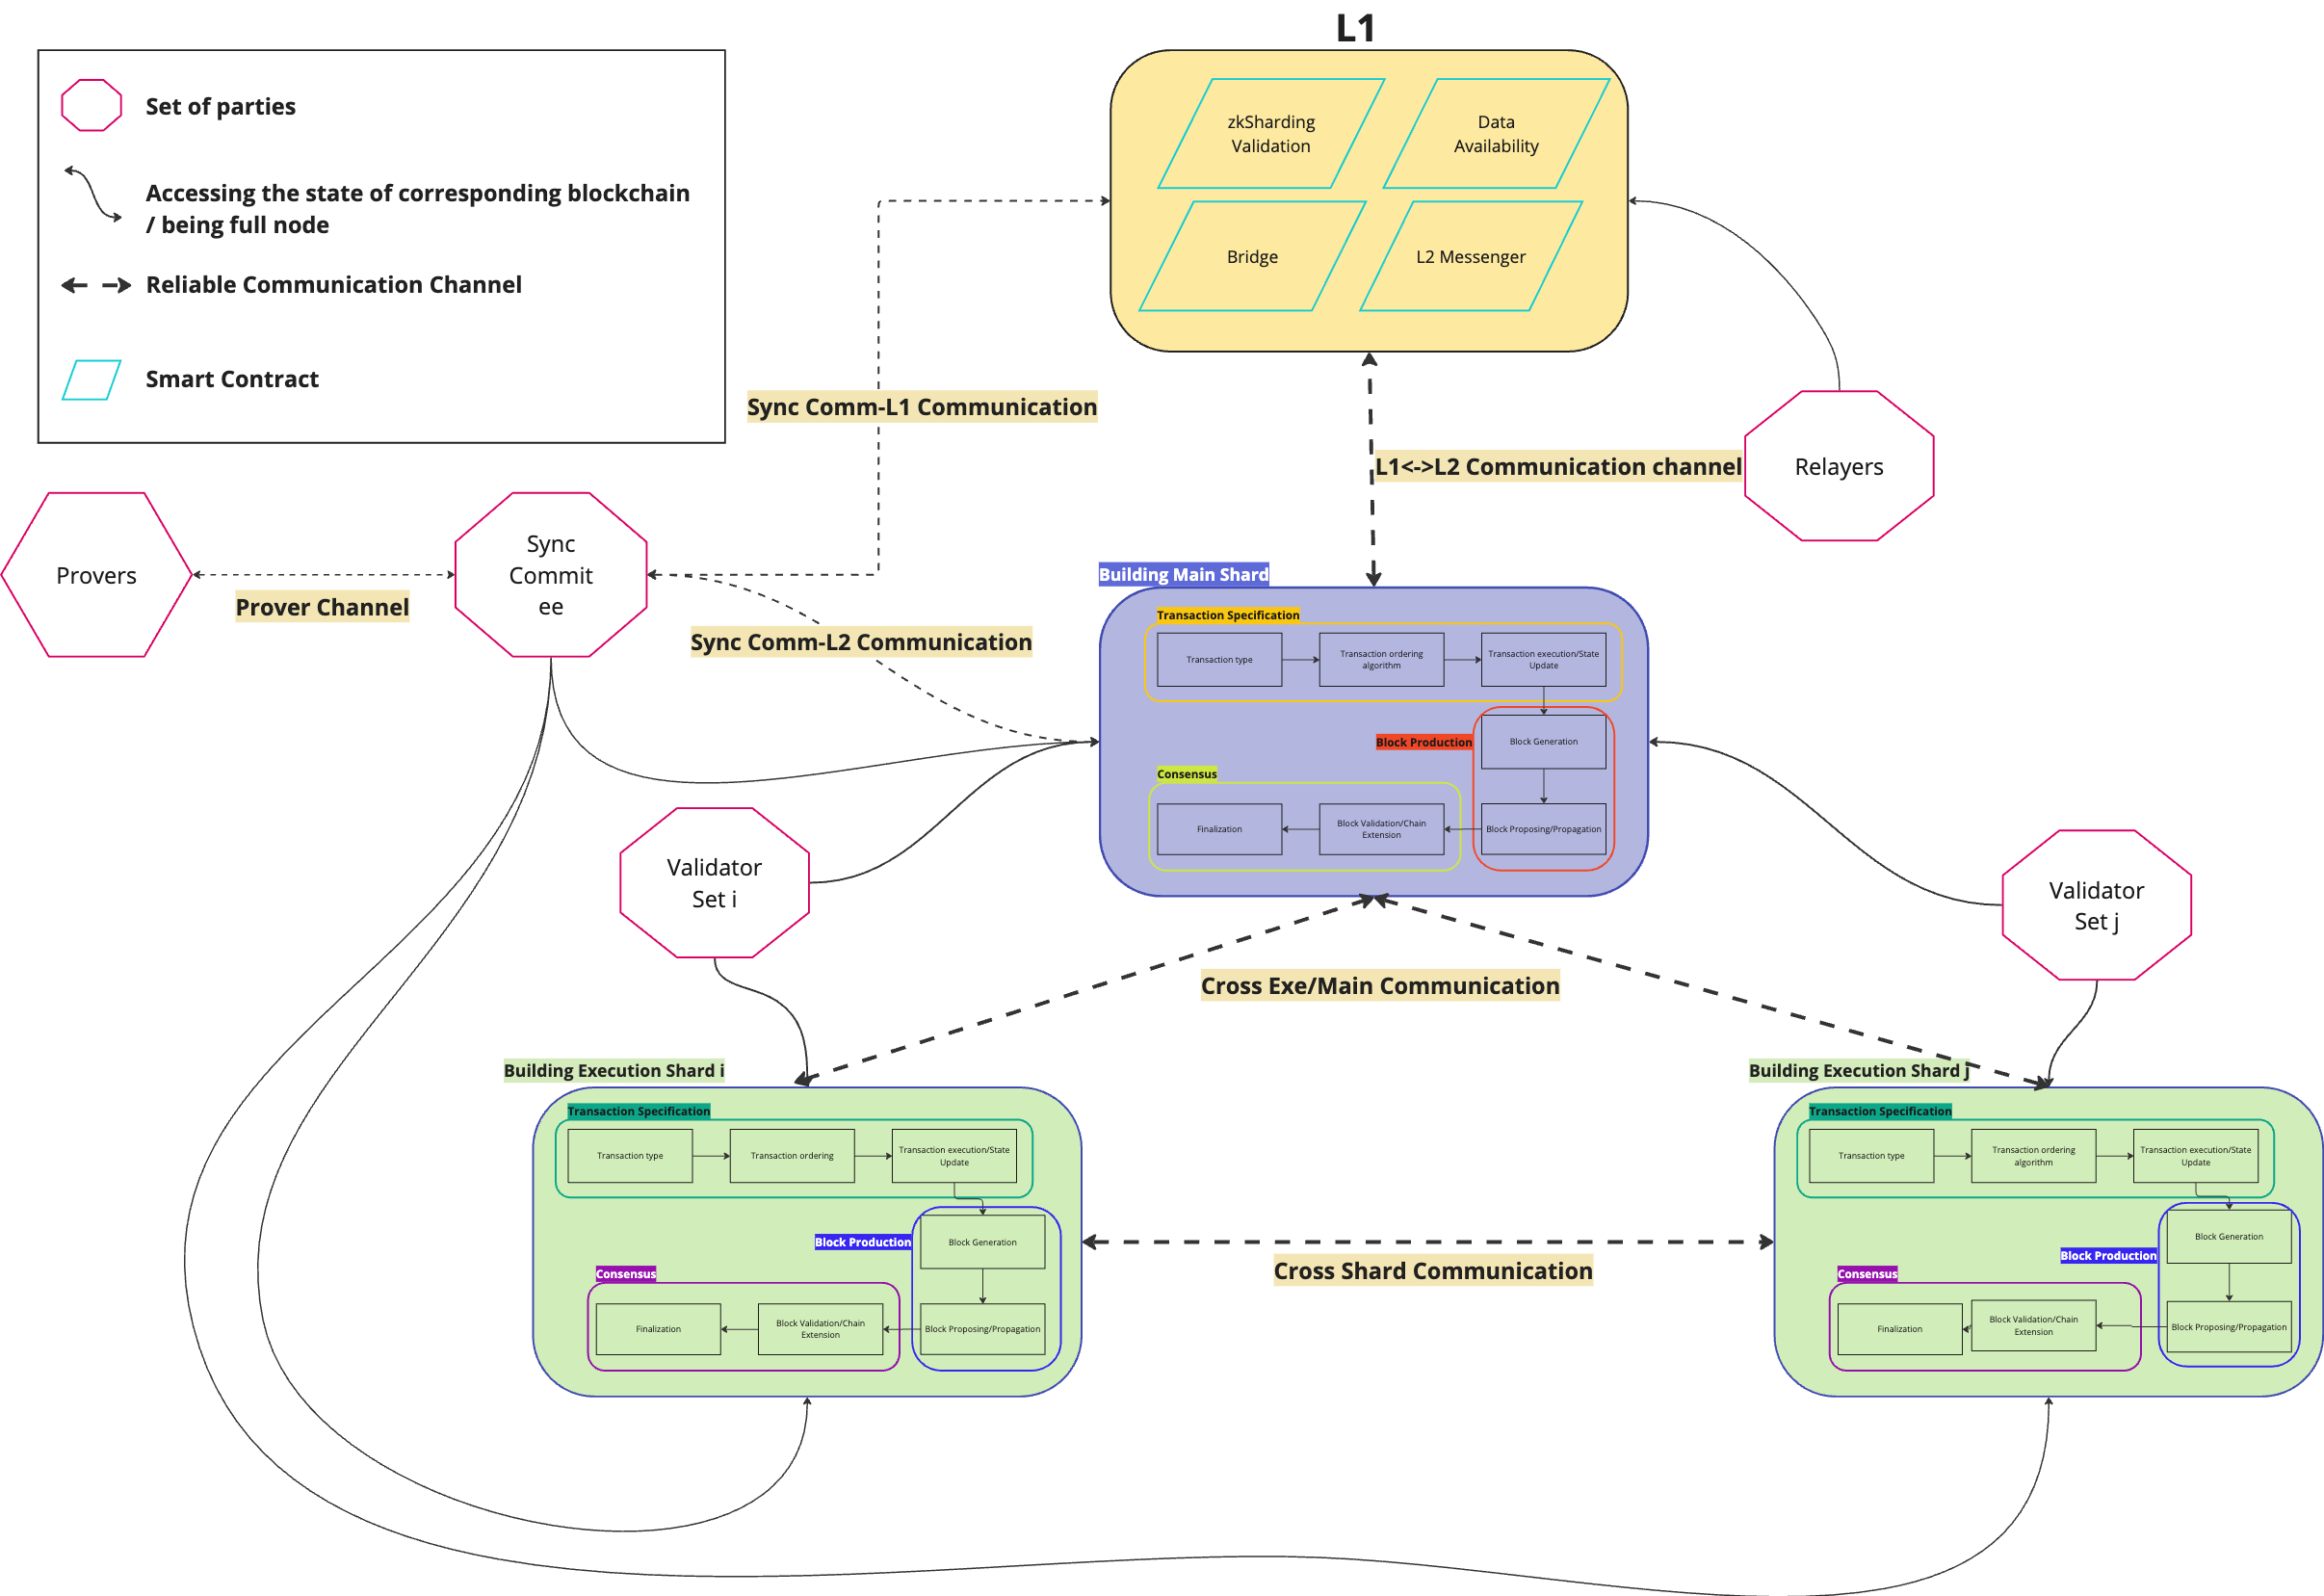
\includegraphics[width=1\linewidth]{figures/components}
%	\caption{zkSharding Components}
%	\label{fig:components}
%\end{figure}
\short{
	As previously discussed, zkSharding operates across three
	interconnected components. Each component serves a distinct
	function, yet they
	work together to ensure  scalability and security. In this
	section, we explore how they are
	linked and describe the architecture that enables state
	synchronization. We
	also introduce the key actors who play critical roles in the
	system.
}{
	As previously discussed, zkSharding operates across three
	interconnected components: L1, the main shard, and multiple
	execution shards.
	Each component serves a distinct function, yet they work together
	to ensure
	scalability, security, and seamless operation of the system. In
	this section, we explore how these layers are
	linked, describing the architecture that enables efficient data
	flow and
	state synchronization. We also introduce the key actors, such as
	validators, provers, and the sync committee, who play critical
	roles in
	maintaining the integrity and security of zkSharding by
	facilitating
	communication and consensus between the layers.
}

\subsection{Actors}

The core participants in zkSharding’s architecture are
\emph{\textbf{validators}}, who play vital roles across different layers.
Each validator $\val_i$ joins the network by staking a certain amount of
funds which incentivizes to maintain the security of the system.
Validators can
operate in multiple roles:

Validators are responsible from building and maintaining the main shard
and execution shards. When operating the main shard, they participate in
running the \emph{global} consensus algorithm which helps to the
synchronization of states across all execution shards.	In the execution
shards, validators are responsible for executing shard-specific
transactions and maintaining its local consensus. Beyond this, validators
can be the part of the synchronization committee $\syncSet$. The members
of $\syncSet$ are responsible for interfacing zkSharding with L1. They
manage tasks like submitting data, proofs, and transactions to the L1
contracts outlined in Section \ref{sec:l1}. The committee is re-elected
each epoch based on protocol parameters, and only validators opting for
this role participate. To maintain clear role separation, a validator
cannot simultaneously serve on both the main shard and the $\syncSet$
committee.

%\begin{itemize}
%	\item \textbf{Main Shard Validators:} These validators are
%	      responsible for building and maintaining the Main Shard. They participate
%	      in running the \emph{global} consensus algorithm that ensures the
%	      synchronization of states across execution shards.
%
%	\item \textbf{Execution Shard Validators:}
%	      \short{
%		      Each execution shard $\shard_i$ has its own set of
%		      validators, $\valset_i$, drawn from the main shard validator set,
%		      $\valset$. These validators are responsible for block creation, executing
%		      transactions, and maintaining \emph{local} consensus in their shard,
%		      $\shard_i$. 
%	      }{
%		      Each execution shard $\shard_i$ has its own subset of
%		      validators, drawn from the main shard validator set $\valset$. We denote
%		      the set of validators specific to an execution shard as $\valset_i$. These
%		      validators are tasked with building blocks, executing transactions, and
%		      running the local consensus mechanism within their assigned execution
%		      shard $\shard_i$. 
%	      }
%
%	\item \textbf{Synchronization Committee:}
%	      \short{
%		      The committee $\syncSet$ is a  group of validators
%		      responsible for interfacing zkSharding with L1. They manage tasks like
%		      submitting data, proofs, and transactions to the L1 contracts outlined in
%		      Section \ref{sec:l1}. The committee is re-elected each epoch based on
%		      protocol parameters, and only validators opting for this role participate.
%		      To maintain clear role separation, a validator cannot simultaneously serve
%		      on both the main shard and the $\syncSet$ committee.
%	      }{
%		      This committee $\syncSet$ is a subset of validators
%		      responsible for interfacing zkSharding with L1. They handle the critical
%		      task of submitting data, proofs, and transactions to the L1 contracts
%		      discussed in Section \ref{sec:l1}. The committee is dynamically elected at
%		      the beginning of each epoch, based on protocol-defined parameters, and
%		      consists of validators who opt into this additional responsibility.
%		      Importantly, to maintain role separation, an account cannot act as both a
%		      main shard validator and a member of $\syncSet$ simultaneously. This
%		      ensures that funds staked by committee members are subject to slashing
%		      only for infractions related to their specific role.
%	      }
%	      By distributing responsibilities across a dynamically elected
%	      group of validators, zkSharding prevents centralization of power, reducing
%	      the risk of collusion or censorship. This ensures the system remains
%	      robust, even if some committee members act maliciously or fail in their
%	      duties.
%\end{itemize}

\short{
	In addition to validators, zkSharding has a role
	\emph{\textbf{prover}}. Each prover $\prover$ is part of a
	dedicated
	proving network and is responsible for executing zkSharding’s
	proving
	algorithm (see Section \ref{sec:zkp}).
}{
	In addition to validators, zkSharding has a role
	\emph{\textbf{prover}}. Each prover $\prover$ is part of a
	dedicated
	proving network and is responsible for executing zkSharding’s
	proving
	algorithm (see Section \ref{sec:zkp}). They generate cryptographic
	proofs
	that verify the correctness of transactions and state transitions,
	which
	are then submitted to validators in $\syncSet$ for further
	processing and
	eventual inclusion on L1.
}
\handan{Should we tell anything about prover fees? Do they get their fee
	from the main shard? Or are they independent actors receiving
	their fee
	from the sync commitee?}

\short{
	Furthermore, there is the role of \emph{\textbf{relayers}}, who
	ensure the reliable transmission of contract calls from Ethereum
	to
	zkSharding.
}{Furthermore, there is the role of \emph{\textbf{relayers}}, who ensure
	the reliable transmission of contract calls from Ethereum to
	zkSharding.
	Relayers facilitate actions such as deposit contract calls,
	guaranteeing
	that messages are reliably delivered to the appropriate components
	within
	zkSharding. This role is integral to zkSharding’s bridge design.
}

\subsection{Components}

In this section, we describe the structure and functionality of the main
shard and execution shards.
\subsubsection{Main Shard:}
Main shard functions as a specialized blockchain that manages operational
transactions crucial to the integrity of zkSharding. The key operational
transactions are as follows:

\begin{itemize}
	\item \textbf{Validator Rotation Algorithm:}
	      Main shard runs a dedicated algorithm, referred to
	      as the
	      \emph{Validator Rotation Algorithm} \cite{rotation},
	      which randomly
	      assigns validators to execution shards. It is
	      optimized to ensure that
	      each execution shard has a sufficient number of
	      honest validators to
	      guarantee safety and reliability.
	      The algorithm divides validators into two groups:
	      large-stake
	      validators (above a set threshold) and smaller-stake
	      validators. It
	      ensures that each execution shard has a balanced
	      representation,
	      prioritizing larger-stake validators for their
	      trustworthiness.
	      Additionally, it enforces a minimum number of
	      validators per shard to
	      promote decentralization and reduce the risk of
	      centralization. This
	      approach maintains fairness, ensuring even
	      distribution of trustworthy
	      validators while guaranteeing that every shard has
	      sufficient validators
	      to operate securely.

	      \begin{enumerate}
		      \item The proportion of large stake validators in
		            each execution shard must be at least
		            $\ratioLexe$.
		      \item The variance in the proportion of large
		            stake validators across all execution shards
		            should not exceed
		            $\distance$.
		      \item Each execution shard must have at least
		            $\lmin$ validators.
	      \end{enumerate}

	      Notably, a validator with a large stake can be assigned to
	      multiple execution shards if necessary.

	      The purpose of the first constraint is to maintain a
	      minimum level of participation from large stake validators,
	      as they are
	      considered more trustworthy. The second constraint ensures
	      that this trust
	      is evenly distributed across multiple shards, avoiding
	      scenarios where a
	      few shards dominate the network. The third constraint
	      prevents
	      centralization by enforcing a minimum validator count for
	      each shard,
	      promoting a more decentralized architecture. More details on
	      the validator
	      allocation algorithm can be found in \cite{}.

	\item \textbf{Randomness Generation:}
	      To support unpredictability outcome of some protocols in
	      zkSharding, the main shard incorporates a
	      randomness generation mechanism.

	\item \textbf{Staking and Slashing:} Validators lock up a certain
	      amount of \emph{stake} when joining the network, which acts
	      as collateral
	      against dishonest behavior. The staking mechanism manages
	      this process,
	      while the slashing protocol penalizes validators for
	      malicious actions.

	\item \textbf{Bridge-Related Operations:}
	      \short{
		      The main shard is responsible for managing
		      operations
		      related to bridging assets and data between
		      zkSharding and Ethereum.
	      }{
		      The main shard is responsible for managing
		      operations
		      related to bridging assets and data between
		      zkSharding and Ethereum. This
		      includes coordinating contract calls, handling token
		      transfers, and
		      ensuring reliable messaging between zkSharding and
		      external blockchain
		      networks.
	      }

	\item \textbf{Finalizing Execution Shard Blocks:} Once an
	      execution shard completes a block, its header is submitted
	      to the main
	      shard, which verifies and finalizes the block header by
	      including it in the
	      global consensus (see Section \ref{sec:globalconsensus})
\end{itemize}

The main shard functions similarly to a referee in a
game.\todois{Comparison creates a feeling of centraliation around main
	shard \handan{How about now?}} Its role is to verify the block
headers from execution shards to validate that each shard adheres to
network rules.	\todois{Technically, it doesn't
	validate the most part of the ES block
	\handan{Done}}
This setup ensures that all execution shards maintain a synchronized view.
It is achieved by the global consensus provided by the main shard.
%Instead, they can
%simply check whether the respective block has been finalized by the main
%shard. This ensures that all execution shards share the same, consistent
%view of the network state.

\short{
	The global consensus in the main shard coordinates and
	synchronizes the states of all execution shards. It provides a
	consistent and
	unified system state. This internal process is distinct from L1
	consensus,
	which validates and finalizes the state of both the main shard and
	execution shards by verifying state validity proofs. While L1
	guarantees
	the validity of zkSharding's state, it is not involved in the
	internal
	synchronization or consensus mechanisms of zkSharding, which focus
	on
	managing shard execution and coordination,
}{
	In more detail, the purpose of global consensus in the main shard
	is to
	synchronize the states across all execution shards. It provides
	consistency
	and agreement on the overall state of the system. Importantly,
	this global
	consensus mechanism is an \emph{internal, operational} process
	within
	zkSharding. It is separate from the L1 consensus.
	The L1 consensus mechanism ultimately finalizes the states of both
	the main shard and the execution shards by verifying the proofs
	that
	zkSharding submits. In this way, L1 ensures that the states of all
	shards
	are valid and finalized, but it is not directly involved in the
	internal
	consensus mechanisms of zkSharding itself,  because the internal
	consensus
	mechanism is related to execution and coordination between
	execution
	shards.
}
In a nutshell, L1 consensus offers an additional layer of protection
through Ethereum’s strong security guarantees. This design combines the
decentralized scalability benefits of sharding with Ethereum's proven
security.
To summarize the consensus layers shown in Figure \ref{fig:consensus}:
\begin{itemize}
	\item Execution shards	run local consensus with their \emph{own
		      validators} to maintain synchronization of their
	      state in the shard.
	\item The main shard runs global consensus with \emph{all
		      validators}, ensuring synchronization and
	      consistency of states across all
	      execution shards.
	\item L1 verifies and finalizes the states of both the main shard
	      and execution shards, ensuring overall zkSharding finality.
\end{itemize}

\begin{figure}
	\centering
	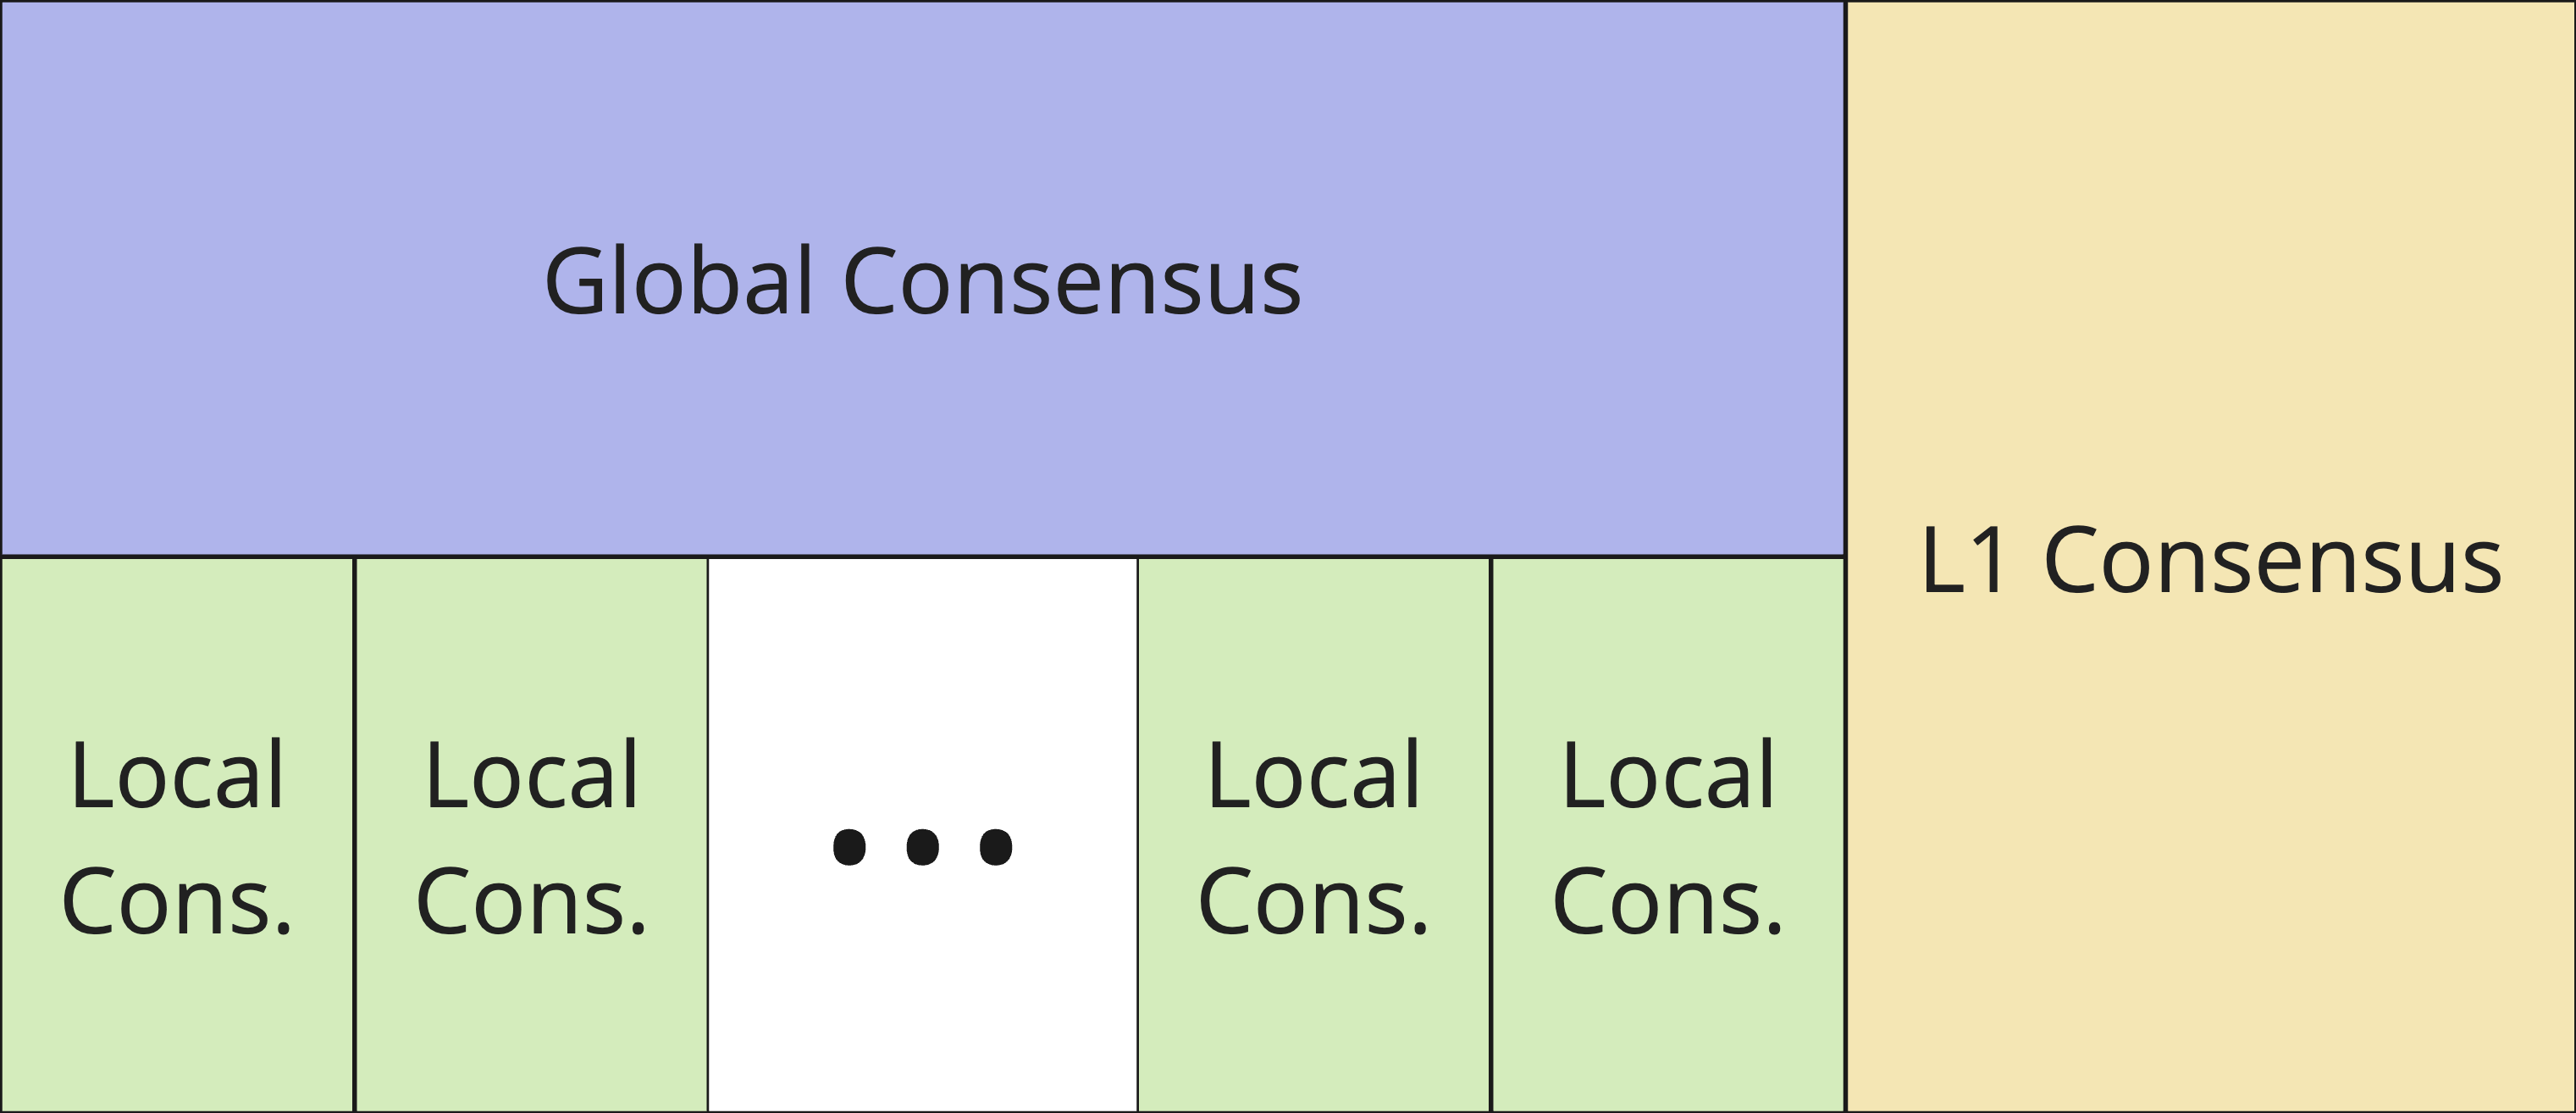
\includegraphics[width=0.5\linewidth]{figures/consensus}
	\caption{Consensus layers in zkSharding: Local consensus aligns
		execution shard states, global consensus by the main shard
		synchronizes
		them, and L1 consensus on Ethereum finalizes the state of
		both main and
		execution shards for overall system security.}
	\label{fig:consensus}
\end{figure}

\subsubsection{Execution Shard}
\label{sec:executionshards}
\todoisinline{The section is not about execution shards but about
	cross-shard comms. We need to include async-related stuff here
	\handan{I added information about acoounts, mempool, message
		delivery, async call, enshrined token design}}
In zkSharding, there are multiple execution shards, each managing its own
set of accounts. An account is the fundamental data unit in each shard and
includes the address, balance, storage root, and a hash of the contract’s
source code. Notably, all accounts in zkSharding are represented by smart
contracts. By structuring all accounts as smart contracts, zkSharding
centralizes operational logic across the system. It simplifies message
handling and state updates.

Each execution shard operates a dedicated mempool that temporarily stores
external messages sent by users, dApps, or other external sources. These
messages are queued in the mempool until the associated smart contract
processes them.
During contract execution, if a contract generates additional internal
messages to other contracts, these bypass the mempool and are instead
routed directly to their target contracts on either the same or another
shard. This direct routing avoids unnecessary queuing, creating a more
efficient and streamlined message processing flow across execution shards.

zkSharding deploys \emph{enshrined token design} \cite{tokenNil} in
execution shards which offers efficient approach to managing token
transaction across execution shards. With enshrined tokens, the core token
functions (like transfer, balance checking, and approvals) are directly
built into the core protocol of execution shards rather than being
implemented through smart contracts. This allows these operations to
benefit from protocol-level optimizations. In this way, the protocol
itself handles the complexity of moving tokens between execution shards.

Execution shards communicate through a
\emph{cross-shard communication protocol}. It guarantees that
messages between shards are
eventually executed. In this protocol, even execution shards which are not
message's
destination play a \textit{supporting} role by storing message-related
data, thereby helping to enforce eventual
execution on the destination shard. \todois{I understand what are you
	trying to explain, but this
	sentense may be more misleading fot the reader \handan{How is it
		now? If it is still misleading, I can remove it}}
To enable efficient communication between execution shards, zkSharding
allow smart contracts deployed on different execution shards to interact
without halting execution. The $\mathtt{asyncCall}$ function
\cite{asyncNil} is integral to this feature. It enables a contract on one
shard to call functions on contracts located on other shards directly,
without waiting for an immediate response. This mechanism produces a
message that is processed by the destination shard asynchronously,
allowing parallelism across shards and improving network scalability.

A unique data structure of our execution shards is the \textbf{ShardDAG}
\cite{sharddagEthResearch}. It is a structure that connects blocks from
different
execution shards as well as blocks from the main shard. This shared
structure imposes a global ordering of transactions that mitigates Maximum
Extractable Value (MEV) attacks \cite{mev1,mev2} especially for
cross-shard
transactions and guarantees ultimate cross-shard transaction processing.

\paragraph{ShardDAG:} It is inspired by DAG-based blockchains
\cite{dagSoK1,dagSoK2}, and operates as
follows:
When a validator generates a block $\block$ for execution shard
$\shard_i$, in addition to the transactions, it adds the following
elements to connect $\block$ to other blocks to form the DAG:
\begin{itemize}
	\item The hash of the latest block from the same shard $\shard_i$,
	      as in a typical blockchain.
	\item Hashes of blocks from other shards, following the ShardDAG
	      rules \cite{sharddag}, which act as acknowledgments that the
	      execution
	      shard has received data from those other shards.
	\item The hash of the latest main shard block to ensure that
	      cross-shard transactions are eventually processed and
	      recognized by the
	      entire network.
\end{itemize}

\begin{figure}
	\centering
	
\includegraphics[width=1\linewidth]{figures/shardDAGStrategy}
	\caption{ The ShardDAG rules enforce a strategy that ensures
		secure cross-shard transactions: (1) \textbf{Child
			Condition} enforces
		data availability by requiring broadcast to more than $F$
		shards; (2)
		\textbf{Parent Condition} guarantees receipt by
		integrating data from
		multiple shards; and (3) \textbf{Main-Parent  Condition}
		maintains order
		with the main shard. Together, these rules ensure secure
		processing and
		reduce exploitation risks.}
	\label{fig:strategy}
\end{figure}

The ShardDAG enforces rules that  are designed to maintain security, data
availability, and orderly processing of transactions. The key rules
include\todois{simplify to less strict definitions \handan{I was not sure
		how to be  less strict so I try to focus more on the
		purpose of the
		rules.}}:

\begin{itemize}
	\item \textbf{Child Condition:} An execution shard block is not
	      finalized until it has received acknowledgments from over
	      $F$ other
	      shards, where $F$ represents the system's tolerance for
	      potentially
	      adversarial shards. This condition helps ensure cross-shard
	      data is
	      sufficiently distributed, preventing single-shard control
	      over transaction
	      flow and supporting broad data availability.

	\item \textbf{Parent Condition:} An execution shard block must
	      have a subgraph that includes blocks from more than $F$
	      other shards
	      relative to its predecessor. This condition encourages
	      regular integration
	      of cross-shard data, reducing the risk of shards bypassing
	      or isolating
	      cross-shard transactions.

	\item \textbf{Main-Parent Condition  \handan{Check the name with
			      James. He refers it as consensus-parent
			      condition}:} A shard block should not
	      reference the same consensus block
	      for more than $X$ consecutive blocks, where $X$ depends on
	      the execution
	      shard's block time. This helps shards stay aligned with
	      updates from the
	      main shard. This promotes synchronization across the
	      network.
\end{itemize}

%LONGER VERSION
%\begin{itemize}
%	\item \textbf{Child Condition:} An execution shard block cannot be
%	      finalized until it is acknowledged by more than $F$ other shards. Here,
%	      $F$ represents the threshold derived from zkSharding’s adversarial
%	      assumptions, specifying the maximum number of potentially malicious shards
%	      that the system can tolerate. This rule ensures that cross-shard
%	      transaction data has been sufficiently broadcast and received across the
%	      network, reinforcing robust data distribution and preventing any single
%	      shard from stalling the transaction flow. By requiring acknowledgments
%	      from multiple shards, the system guarantees that cross-shard data
%	      availability is maintained.
%
%	\item \textbf{Parent Condition:} For an execution shard block to
%	      be considered valid, the graph difference between its subgraph and the
%	      subgraph of its previous block must contain blocks from more than $F$
%	      different shards.  This rule prevents any shard from bypassing the
%	      processing of cross-shard transactions or selectively isolating
%	      transactions, as it compels each shard to integrate data from multiple
%	      other shards, ensuring that cross-shard transactions are acknowledged and
%	      processed.
%
%	\item \textbf{Main-Parent Condition \handan{Check the name with
%			      James. He refers it as consensus-parent condition}:} A shard block is only
%	      considered valid if it has not created more than $X$  consecutive blocks
%	      referencing the same consensus block. The parameter $X$ depends on the
%	      block time of an execution shard. This rule ensures that shards stay
%	      synchronized with the main shard’s state and prevents any shard from
%	      endlessly producing blocks that do not account for new information from
%	      the main shard. This condition enforces consistent synchronization across
%	      the network.
%\end{itemize}

\short{
	See Figure \ref{fig:strategy} for a detailed illustration of how
	these rules enforce constraints for succesfull and orderly
	execution of
	transactions.
}{
	By enforcing these ShardDAG rules, zkSharding guarantees that
	cross-shard transactions are processed securely, efficiently, and
	in an
	ordered manner. See Figure \ref{fig:strategy} for a detailed
	illustration
	of how these rules enforce constraints for successful
	execution.These
	rules also help to mitigate the risks of MEV exploitation and
	censorship,
	ensuring that malicious behavior cannot manipulate or delay
	transactions.
}

%
%\paragraph{Prover Network:}
% Provers in the zkSharding system are responsible for generating zkps for the entire batch of transactions and state updates. Each proof certifies that the state transitions within the batch are valid and that no malicious changes were made. Once generated, the proofs are sent back to the sync commitee.
\section{Transaction Lifecycle: From Execution to L1 Finality}
\label{sec:txlifecycle}

In this section, we describe the lifecycle of a transaction in zkSharding,
while highlighting specific solutions introduced to ensure both security
and efficiency.

In zkSharding, there are two fundamantal messages: external and internal
\handan{Does the naming make sense?}.  External messages originate from
external actors and are sent directly to the mempool of the contract’s
execution shard for processing. Internal messages, on the other hand, are
generated during contract execution and do not enter the mempool, as we
explained in Section \ref{sec:executionshards}. We differenciate internal
messages, for the sake of clarity in this section, as intra-shard
transactions (ISTs) and cross-shard transactions (CSTs) although ISTs and
CSTs share  the same structure and follow the similar execution path in
zkSharding.

Each internal message contains several fields that help process it
robustly,
but the key distinction between ISTs and CSTs lies in two specific fields:
the sender contract address $\sender$ and  the recipient contract address
$\to$.	To differentiate between shards, we use superscripts to denote
which shard the accounts belong to, e.g.,  $\sender^i$ and $\to^i$
indicate that  the sender or recipient account belongs to execution shard
$\shard_i$.
For a given transaction $\tx = (\sender^i, \to^j)$, if $i = j$, meaning
both the sender and recipient belong to the same shard, we classify it as
an \emph{intra-shard transaction (IST)}. If $i \neq j$, where the sender
and recipient belong to different shards, we classify it as a
\emph{cross-shard transaction (CST)}. In short:
\begin{itemize}
	\item ISTs are processed entirely in the execution shard where
	      they are initiated.
	\item CSTs involve interaction between different shards and
	      require cross-shard coordination.
\end{itemize}

Once either an internal or external message arrives to the execution
shard, it waits to be included in a block by a
block producer, who connects it to the blockchain, making it a canonical
part of the execution shard. Below, we describe this process in the
context of a block producer of $\shard_i$.

\subsection{Reaching Local Consensus}

\begin{figure}
	\centering
	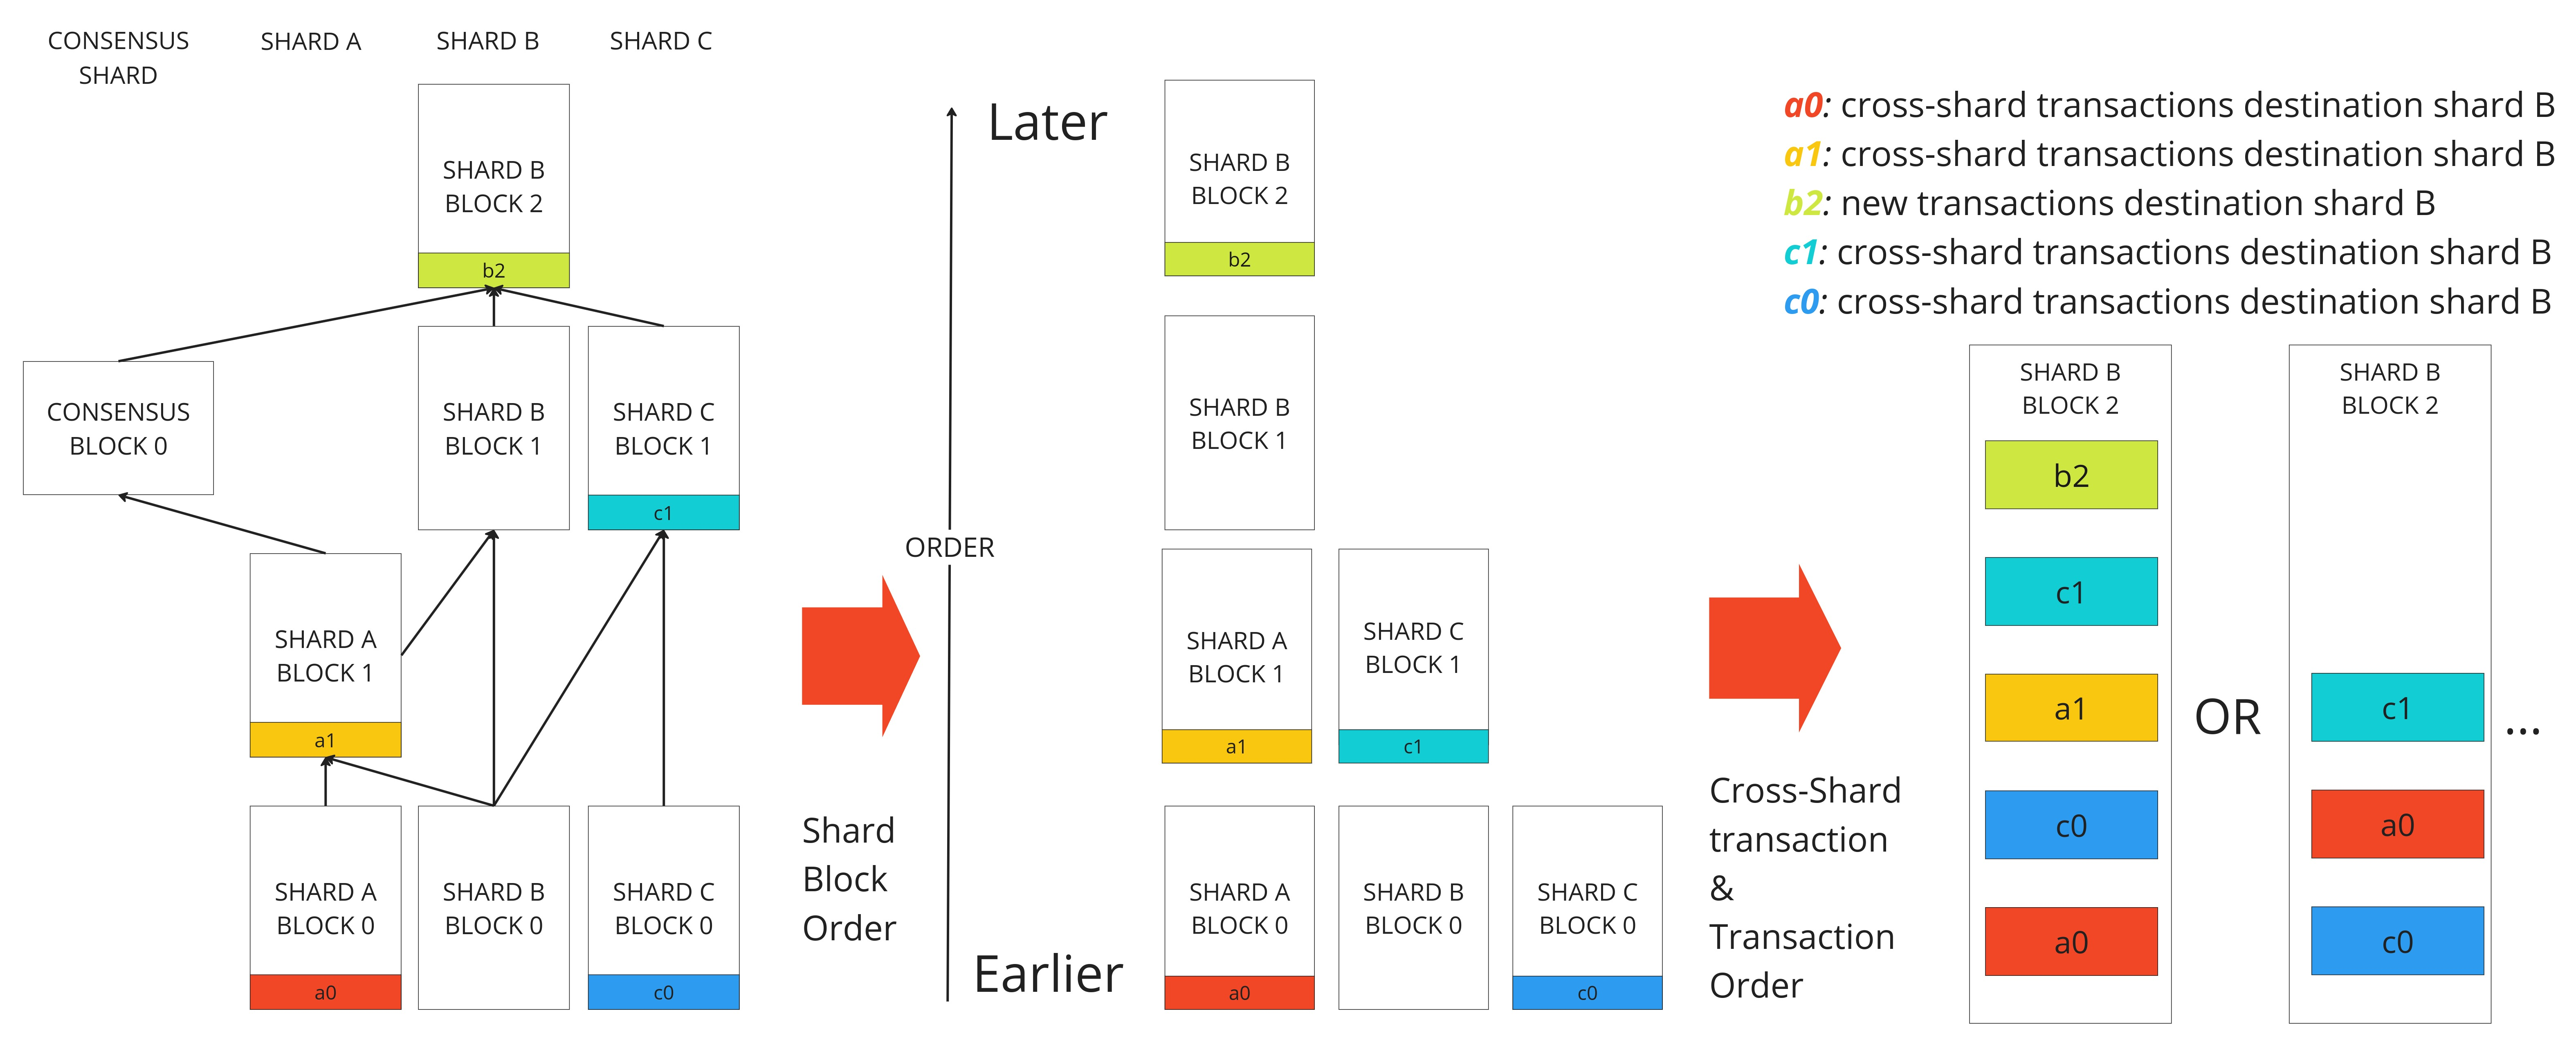
\includegraphics[width=1\linewidth]{figures/OrderExample}
	\caption{ShardDAG Order \handan{change notation and namings}}
	\label{fig:order}
\end{figure}
\begin{itemize}
	\item \textbf{Transaction ordering:}.
	      %, following transaction
	      %ordering rules based on factors such as \emph{fee}, \emph{priority},
	      %\emph{transaction type}, and  the \emph{ShardDAG ordering rules}.
	      The block producer begins by applying the ShardDAG ordering
	      rules (see Figure \ref{fig:order}). For this,
	      it first analyzes the local shardDAG subgraph for shard
	      $\shard_i$. This subgraph contains unprocessed transactions
	      $
		      \{(\sender^j, \to^i)\}$ where $j = i$ or $j \neq i$
	      and their dependencies
	      across different execution shards. The block producer then
	      determines the
	      order of these transactions with the help of the subgraph.
	      In case additional block space is available, it also selects
	      a set of
	      transactions from the mempool. In the end, it obtains the
	      list of transactions $\txlist$ to be processed.
	      The ShardDAG ordering rules enforce a \textit{parent-child
		      relationship} between transactions to be processed
	      in a valid order.
	      Specifically, CSTs with earlier dependencies must be
	      processed before
	      later transactions. This ordering prevents inconsistencies
	      in cross-shard
	      interactions.

	\item \textbf{Block Creation:} The proposer executes all
	      transactions in $ \txlist $ in the context of the latest
	      state using the
	      state transition function. If these executions
	      result in new cross-shard transactions
	      (CSTs), such as $ (\sender^i, \to^j) $ where $ i \neq j $,
	      the proposer
	      adds them to a special data structure called the
	      \emph{outbox} $ \outbox_i
	      $. $ \outbox_i $ tracks all CSTs originating from $ \shard_i
	      $ that are
	      waiting to be processed by their respective destination
	      shards\footnote{If
		      the block capacity is full and the mempool still
		      contains unprocessed messages  that should be
		      included based on the
		      ShardDAG order, they can be
		      added to the block's outbox for future inclusion in
		      later blocks
		      \cite{sharddag}}.

	      After executing the transactions, the block producer creates
	      a
	      block $ \block $. We note that if the execution of some CSTs
	      and ISTs fails, they enter a refund mechanism that allows
	      failed
	      transactions to be retried with additional fees or canceled
	      via the
	      mailbox.

	      \handan{It is not clear what solutions we use for the
		      failed CSTs. I am not sure whether what I wrote is
		      corret or not.}
	      When bulding $\block$, the block producer respects to the
	      Parent and Main-Parent condtions of ShardDAG rules.
	      Therefore, it
	      retrieves any new outgoing CSTs from other execution shards
	      and includes
	      the hashes of the originating blocks in $\block$, thereby
	      linking $\block$
	      to the corresponding blocks from other execution shards.
	      $\block$
	      includes the list of executed transactions $
		      \txlist $, the updated state $ \st $, state root
	      $\stroot$ of
	      $\st$, the outbox $ \outbox_i $, which contains CSTs that
	      are yet to be
	      processed by other shards and block header $\bhead$. This
	      newly created block is then proposed to
	      the network as part of the local consensus process.

	\item \textbf{Local Consensus:} After receiving the block $ \block
	      $, the validators initiate the Multi-Threshold BFT
	      \handan{Should we give the name of the consensus mechanism?
		      Maybe we
		      should not since it might change}
	      consensus mechanism \cite{MultiThresholdBFT} to validate and
	      finalize the
	      block \emph{locally} within execution shard $ \shard_i $.
	      Each validator
	      verifies the block’s correctness by \footnote{The list of
		      checks is not
		      exhaustive. We give the critical ones ensuring the
		      safety and security of
		      cross-shard communication.}
	      \begin{itemize}
		      \item verifying  the correctness of the transaction
		            order
		            in $\block$ to ensure that the order of
		            transactions adheres to the rules
		            of the shardDAG,
		      \item verifying if the block follows the parent
		            condition
		            and main-parent condition introduced by
		            ShardDAG rules and,
		      \item checking if $\fstf(\st', \txlist) \rightarrow
			            \st $
		            where $\st'$ is the last locally finalized
		            state.
	      \end{itemize}
	      Once a supermajority of validators  agrees on the
	      block's validity, the block is finalized locally.
	      This local consensus ensures that the block is securely
	      added to
	      $\shard_i $'s chain while maintaining consistency with the
	      shardDAG
	      ordering rules.
	      \short{
	      }{
		      The finalized block's header can then be propagated
		      to
		      other shards for further processing of CSTs as
		      described next.
	      }
	\item \textbf{Block Propogation:} After $\block$ is finalized
	      locally, validators are responsible for distributing $
		      \outbox_i $ and $ \bhead $ to the destination shards
	      $ \shard_j $, as well
	      as to other shards to ensure data availability of CSTs. They
	      are
	      incentivized to propagate the data to help reaching global
	      consensus at
	      the main shard level, as required by the child condition.
	      Remember that execution shards that receive the CST data
	      link
	      their next block to $ \bhead $. Even shards that do not
	      process the CSTs
	      must store the data off-chain, as they may be involved in
	      forming DAG
	      edges or verifying the ShardDAG rules, which is essential
	      for their own
	      block finality.

\end{itemize}

Validator sends $\bhead$ to the main shard after finalizing
it locally.

\subsection{Reaching the Global Consensus}
\label{sec:globalconsensus}

When the main shard validators receive a block header $\bhead$ from an
execution shard, they perform the following checks before including
$\bhead$ in a main shard block:

\begin{itemize}
	\item \textbf{Local Finality Check:} Confirm that $\bhead$ has
	      been signed by a supermajority of validators, indicating
	      that it has achieved local finality.
	\item \textbf{Validation of ShardDAG Rules:} Verify that the
	      \emph{Parent Condition}, \emph{Child Condition}, and
	      \emph{Main-Parent
		      Condition} are all satisfied. If
	      any of these conditions fail, the validators who signed
	      $\bhead$ are subject to slashing penalties.
\end{itemize}

If all checks pass, $\bhead$ is included in a main shard block and
finalized. If some of the checks are not passed, the validators signed for
$\bhead$ are slashed.

%However, at this stage,
%$\bhead$ is not yet fully recognized as a canonical part of $\shard_i$'s
%state because its state transition needs to be further verified.

%Once the synchronization committee (explained in the following section)
%submits a valid proof for a batch $\batch$ of transactions processed
%across all execution shards, the main shard validators update the status
%of $\bhead$ which has transactions in $\batch$ to \emph{finalized}. This
%step completes the process of achieving global consensus for $\bhead$ on
%$\shard_i$.
%
%Execution shards observing a pending $\bhead$ can infer that the CSTs
%included in the outbox of the block were correctly constructed according
%to ShardDAG rules and that the validators have agreed on
%the correct construction of the state. Thus, they can optimistically trust
%that $\stroot \in \bhead$ accurately represents the correct state $\st$
%without waiting for $\bhead$ to achieve global consensus on the main shard
%to process the CSTs.
%
%Our rotation algorithm, along with the high safety threshold of Multi-BFT,
%ensures that the safety of an execution shard is highly unlikely to be
%compromised. However, even in the rare case of a safety violation, we
%implement a rollback mechanism that ensures execution shards can revert to
%an uncorrupted state. Given the low probability of safety violations and
%the economic disincentives against attacking an execution shard, execution
%shards can rely on pending block headers to maintain continuity in their
%operations.

\subsection{Reaching the L1 Finality}

With the transactions now executed in an execution shard block and
included in the main shard, the next step involves the synchronization
committee $\syncSet$ to extract the transaction data, coordinate with
provers to generate proofs, and ultimately submit the verified data to L1
for final settlement and verification.
%In zkSharding, we have subset of validators that we call synchronization committee. This committee takes charge of extracting the transaction data, coordinating with provers to generate zk-proofs, and ultimately submitting the verified data to L1 for final settlement and verification. It is responsible for ensuring that the state changes and transactions from the execution shards are ready to be validated and posted to L1. 
Here is how  $\syncSet$\todois{not enough info on SC in the doc
	\handan{What else can I add? Maybe a motivation why we have such
		separate
		mechanism for it?}} executes
the process:

\begin{itemize}
	\item The \textbf{observer}\todois{From the text, it's not clear
		      what is the entity "observer" \handan{Not clear what
			      is not clear}} in $\syncSet$ monitors the
	      growth of the
	      main shard's state and execution shard states. Once the
	      state changes
	      reach a certain threshold, the observer initiates the
	      process of preparing
	      data for L1 submission.
	\item When the observer signals that a snapshot of data between
	      time $T$ (just after the last proven state) and $T + n$ is
	      ready, the
	      \textbf{aggregator} in $\syncSet$ compiles the data executed
	      between $T$
	      and $T+n$ in \emph{all} shards into a batch. Each batch of
	      $\shard_i$ consists of
	      transactions $\txlist_i$ executed between time $T $ and
	      $T+n$.
	      Addionally, the batch of the main shard consists of list of
	      transactions $\txlist_M$
	      between time $T$ and $T+n$ related to
	      % bridge operations such as
	      %withdrawal, depositing or 
	      validator operations such as staking, slashing
	      which are related the security of the internal sharding
	      mechanism. In the
	      end, aggregator composes	$k+1$ bathches where $k$ is the
	      number of
	      execution shard into one batch $\batch$.
	      The aggregator sends $\batch$, the last verified state on L1
	      $\st'$, and other necessary data to the verifier	in
	      $\syncSet$. It also forwards $\batch$ to the
	      proposer in $\syncSet$.
	      By grouping all transactions into a batch, we achieve better
	      cost-efficiency during the proving process.
	\item The \textbf{verifier} generates a special transaction called
	      \emph{proof order} to outsource the proof generation process
	      to the prover
	      network.	The proof order specifies the batch and state
	      updates that need
	      to be proven, along with a payment for generating the proof.
	      Prover
	      network runs the proving algorithm which receives as a
	      private input
	      $\batch$, current state $\st'$ and as a public input
	      %$\combatch$ which is
	      %the commitment of $\batch$ and 
	      the new state root $\stroot$ and previous
	      verified state root $\stroot'$. In simple terms, provers
	      generate a succinct proof $\pi$ that verifies the
	      correctness of the new
	      state with the public inputs (See Section \ref{sec:l1} to
	      understand the
	      proving statement).

	      %	       (part of) our proving
	      %	      system runs for the following relation $\mathcal{R}_\fstf$:
	      %
	      %	      \begin{align*}
	      %		      \mathcal{R}_\fstf = & \{((\batch, \st'); (\combatch,
	      %		      \stroot, \stroot')):  \mtroot(\st) \rightarrow \stroot, \mtroot(\st')
	      %		      \rightarrow \stroot'                                                      \\ \nonumber
	      %		                          & \fstf(\st',\batch) \rightarrow \st, \commit(\batch)
	      %		      \rightarrow \combatch \}
	      %	      \end{align*}
	      %
	      %	      where $\commit$ is a commitment algorithm and $\mtroot$ is an
	      %	      algorithm that outputs the Merkle Tree root of a given state.
	      %	      In the end, our proving algorithm outputs a proof $\pi$ if
	      %	      $((\batch, \st'); (\combatch, \stroot, \stroot')) \in \mathcal{R}_\fstf
	      %	      $. 
	      After receiving $\pi$, the verifier gives
	      $\pi$ to the proposer if $\pi $ is verified.
	      The provers joining the proving process get their fee.
	\item The \textbf{Proposer} runs the compression algorithm
	      for $\batch$ which is an optimized algorithm
	      for zkSharding’s specific data types (e.g., block headers,
	      state roots,
	      and transaction summaries). This reduces the size of the
	      data submitted to
	      L1. Once the batch is compressed, the proposer submits it to
	      L1 through an
	      EIP-4844 blob transaction. This transaction includes the
	      compressed batch
	      data. The blob transaction ensures that the data is
	      permanently
	      stored and its KZG commitment $\kzg$ is accessible for
	      future
	      verification.
	      Addionally, the proposer submits $\pi$ and public inputs to
	      the
	      L1 state validity contract and the main shard.
\end{itemize}

Once the L1 State Validity Contract verifies $\pi$ as described in Section
\ref{sec:l1}, it updates the verified state root to $\stroot$ and
finalizes it as part of L1 through Casper FFG. It means that once a state
is finalized  through Casper FFG, it is irreversible and considered as a
canonical part of  Ethereum and also zkSharding.

\handan{Add motivation why we have distinct roles within the sync
	commitee, why do we we have many members, how the roles are
	distributed.}
\section{Proof Sytem in zkSharding}
\label{sec:zkp}
Our zkEVM \cite{zkevm} operates at the bytecode level by directly
interpreting EVM bytecode. It  ensures high compatibility with existing
Ethereum dApps and smart contracts, although it may produce slightly
different state roots than the standard EVM due to the use of
SNARK-friendly optimizations. Projects like Scroll \cite{scroll} and
Hermez \cite{hermez} by Polygon also use this method.

In our zkEVM, we use FRI-based placeholder proof system \cite{placeholder}
which uses  lookup argument \cite{plookup}.  During the implementation of
Plookup and its practical use, we encountered some technical issues that
were not mentioned in the original solution. Therefore, we propose
practical improvements \cite{plookuptweaks} for writing large PLONK
circuits with a complex logic.

zkSharding’s zkEVM consists of multiple subcircuits\todois{ref to PSE
	solution}, each of which is handled by separate provers. A
straightforward
approach would be to have each prover $\prover_i$ generate an independent
FRI-based proof $\pi_i$ for each subcircuit $\circuit_i$, resulting in $M$
proofs (where $M$ is the number of subcircuits). These proofs would then
need to be aggregated into a succinct proof $\pi$. However, FRI lacks
homomorphic properties, making this aggregation process computationally
expensive, which contradicts FRI's main advantage of prover efficiency.

To address this, we designed Distributed FRI (DFRI) \cite{dfri}, which
uses FRI batching techniques to enable efficient proof aggregation across
multiple provers. In DFRI, the committed polynomials from each prover are
combined using a collaboratively generated random challenge. This batching
mechanism allows us to aggregate the proofs more efficiently while
maintaining the security and integrity of the proof system. DFRI also
ensures accountability by making dishonest behavior from any prover
detectable, which is crucial for maintaining liveness in distributed
systems like zkSharding.

From a performance perspective, DFRI maintains the same proof size as a
single FRI proof, as compared to the straightforward approach which would
involve having $M$ proofs without infeasable aggregation layer. This is
achieved through coordination between provers during the proving process
by slightly increasing the communication overhead. Additonally, DFRI does
not extend the overall proving time comparing to the single FRI-based
prover.
Overall, DFRI helps retain the efficiency of FRI while enabling secure,
distributed proof generation, making it a critical innovation for
zkSharding's scalability and security.
\section{Local Fee Model}
\alex {Do we need more detail or any examples?}

In zkSharding, gas price calculation follows a Local Fee Model at the shard level. Each shard maintains its own distinct base fee, designed to regulate gas demand and promote balanced load distribution across the network.

\subsection{zkSharding Transaction Fee Mechanism}

The zkSharding transaction fee mechanism consists of several key components:

\begin{itemize}
    \item \textbf{Shard-Specific Base Fees}: Each shard operates with its own independent base fee, enabling granular control over gas demand and encouraging an even workload across the network.

    \item \textbf{Adjustment Mechanism}: The model incorporates a modified EIP-1559 base fee adjustment mechanism designed for quicker adjustments during periods of high congestion, enabling shards to dynamically adapt their base fees to prevailing network conditions. In addition to faster responsiveness, the mechanism allows greater flexibility around the target gas usage, aiming to enhance the predictability of cross-shard transactions and transaction fees when the system is in a balanced state.

    \item \textbf{Fee Credit}: To address the variation in base fee levels across shards and the complexity of tracking gas usage for cross-shard transactions, particularly in ensuring messages adhere to gas limit constraints, we use the Fee Credit approach. This Fee Credit is set at transaction creation and is a result of:  \( \text{GasLimit} \times \text{maxFeePerGas} \).
    
    \item \textbf{Propagating maxFeePerGas and maxPriorityFeePerGas values}: Although transactions pay for gas using the Fee Credit, we propagate these two fields to maintain a familiar fee-charging experience. This approach prevents validators from always claiming the full maxPriorityFeePerGas by deriving an effectivePriorityFee. Additionally, it allows users to set an explicit cap on the maximum price they are willing to pay per gas unit, ensuring greater control over transaction costs.
    
    \item \textbf{Fee Credit Forwarding}: As transactions can create new cross-shard transactions we introduce Fee Credit forwarding. \alex {More details needed about forwarding?}
    
    \item \textbf{EMA-Based Smoothing}: To address volatility in L1 blob base fees, the model uses an Exponential Moving Average (EMA). This smooths out fee spikes by distributing their impact over time, preventing sudden cost increases for users.

    \item \textbf{Transformation of L1 Fees into Gas}: L1 fees, such as those for data availability and proof verification, are converted into gas units added to the recomended gasLimit to maintain compatibility with Ethereum’s existing tools and frameworks.  These gas units are excluded from the base fee adjustment mechanism, ensuring a clear separation between L1 fee and L2 fee dynamics.
\end{itemize}
\section{Conclusion}
zkSharding presents a robust solution to Ethereum's scalability challenges by leveraging sharding and SNARK-based proofs. By dividing the network into execution shards and synchronizing their state via the main shard, zkSharding ensures efficient, decentralized processing without fragmenting liquidity. Ethereum serves as the settlement and data availability layer, further enhancing the system's security. Through techniques like DFRI and a multi-layer consensus model, zkSharding achieves a balance between scalability, security, and decentralization, making it a promising framework for Ethereum’s future.






\addcontentsline{toc}{chapter}{\bibname}
\bibliography{biblio}
\nocite{*}


\appendix

% \section{Pacemaker Subprotocol}
\label{appendix:pacemaker}

\todo[inline]{committee changes and pacemaker synchronization with new committees are yet to be detailed}
\todo[inline]{add fail scenarios and timeouts description}

Here we describe the pacemaker subprotocol, which is responsible liveness of the system.
This protocol guarantees that the system makes progress, i.e., it guarantees that the honest nodes will
eventually enter the same view with the correct leader for a sufficient amount of time.

We provide a high-level description of the simplified Version of Naor-Keidar protocol, called Cogsworth \cite{Cogsworth}, in Algorithm \ref{alg:pacemaker-protocol}.


\SetKwInput{KwWish}{WISH}
\SetKwInput{KwReady}{READY}
\SetKwInput{KwAdvance}{ADVANCE}

\begin{algorithm}[H]
    \DontPrintSemicolon
    \SetAlgoLined
    \caption{Pacemaker Protocol (Cogsworth)}
    \label{alg:pacemaker-protocol}
    \SetKwProg{Step}{Step}{:}{}
    \Step{Wish}{
        \textbf{Non-Leader:} If there is no progress, send the leader of view \( r+1 \) a message \( \texttt{(WISH, r+1)} \).

        \textbf{Leader:} Collects \( f+1 \) \( \texttt{(WISH, r+1)} \) messages and broadcasts an aggregate.
    }
    \Step{Ready}{
        % Byzantyne reliable broadcast is just broadcast, collect 2f+1 votes and broadcast again
        Upon receiving \texttt{WISH} aggregate from any leader, it responds with \( \texttt{(READY, r+1)} \).\;

        Upon timeout, it forwards the \texttt{WISH} aggregate to fallback leaders of views \( r+2, \ldots, r+f+1 \), one by one, to collect READY responses, until there is progress.
    }
    % advance
    %  - C(C(B)) is collected, then enter the next view (optimistic case)
    \Step{Advance}{
        \textbf{Leader:} \( 2f+1 \) \( \texttt{(READY, r+1)} \) messages and broadcasts a \texttt{READY} aggregate.\;
        \textbf{Non-Leader:} Upon receiving a \texttt{READY} aggregate from any leader, it enters view \( r+1 \).
        Upon timeout, it forwards the \texttt{WISH} aggregate to fallback leaders of views \( r+2, \ldots, r+f+1 \),
        one by one, to collect \texttt{READY} responses, until there is progress.
    }
\end{algorithm}

% \section{Leader Election Subprotocol}
\label{appendix:election}

One could rotate leaders in a round-robin fashion, $\texttt{leader\_id} = \texttt{view} \mod n$,
but this would be vulnerable to DoS attacks, since an adversary easily can obtain the leader schedule.
Instead, we use a leader election protocol based on Verifiable Random Functions (VRFs), as proposed in \cite{LibraBFT}:
\begin{align*}
    \texttt{seed} &= \texttt{VRF}_{\texttt{prev\_leader}}(\texttt{height}, \texttt{view}) \\
    \texttt{leader\_id} &= \texttt{PRF}_{\texttt{seed}}(\texttt{view}) \mod n
\end{align*}
where \texttt{PRF} is a pseudorandom function.
The leader of the previous view provides the seed as a result of evaluating the VRF.
Every node can verify that the seed is correct by evaluating the VRF with the public key of the previous leader.

%-------------------------------------------------------------------------------

\end{document}